%!TEX root = ../main.tex

\chapter{Response of an event-based camera\label{chap:response}}

\section{Event-based cameras compared to frame-based cameras}

Traditional frame-based (sometimes called global shutter) cameras capture the scene as a sequence of still image frames at fixed intervals with fixed settings, providing a synchronous representation of the visual world. 
In terms of ease of use and the simplicity of the post-processing of data obtained from such cameras, they are wildly applicable across many fields.
A single frame obtained from a frame-based camera may be described by the following equation \refeq{eq:frame} \cite{scheerlinck2018event}
\begin{equation}
Y_j(\boldsymbol{p}) := \frac{1}{\epsilon} \int_{t_j - \epsilon}^{t_j} Y(\boldsymbol{p}, \tau) \mathrm{d} \tau, \quad j \in 1, 2, 3 ...
\label{eq:frame}
\end{equation}
where $Y(\boldsymbol{p}, t)$ denotes the irradiation intensity of a camera pixel at a specific time $t$, $t_j$ is the time-stamp of the image capture and $\epsilon$ is the exposure time.
As we can see, each frame is represented by a temporal average of irradiance over the exposure time $\epsilon$. Although this model simplifies image formation, it introduces artifacts such as motion blur, particularly when fast-moving objects are captured with an exposure time mismatched to their dynamics.

\ac{DVS} (or event-based cameras), are vision sensors that draw their inspiration from nature bio-receptors, where each pixel reacts
to the change of illumination in the scene. Each pixel individually recognizes the log intensity and compares it to the previously
recorded value. When a predefined threshold is crossed, this value is reset to the current one and a new event is generated. This event can be expressed as $e = \begin{bmatrix} x & y & \sigma & t \end{bmatrix}$, where $\begin{bmatrix} x & y \end{bmatrix}$
is the camera pixel coordinate, $\sigma$ is the polarity of change (where $\sigma = \pm 1$ for increasing or decreasing change, respectively) and $t$ is the timestamp of the event. \cite{gallego22event} \cite{scheerlinck2018event} We can model the single event as a Dirac-delta function $\delta(t)$ and can define an event stream
$e_i(\boldsymbol{p}, t)$ at a pixel $\boldsymbol{p}$ by \refeq{eq:event_eq} \cite{scheerlinck2018event}
\begin{equation}
e_i(\boldsymbol{p}, t) := \sigma_i^{\boldsymbol{p}} c \, \delta(t - t_i^{\boldsymbol{p}}), \ i \in 1, 2, 3 ...
\label{eq:event_eq}
\end{equation}
where $\sigma_i^{\boldsymbol{p}}$ is the polarity (sometimes referred simply as an ON or OFF event) and $t_i^{\boldsymbol{p}}$ is the time-stamp of the $i$-th event at a pixel.
The magnitude $c$ is the contrast threshold, a preset constant (similar to exposure time in frame-based cameras), which defines a change in light intensity that is encoded by a singular event, at each pixel. Event-based cameras thus circumvent many common issues found in traditional frame-based cameras, such as the motion blur mentioned before. They offer significant advantages, including high dynamic range, low latency,
and energy efficiency.
This makes them perfect for the application of agile robotics,
where the fast response time is crucial (especially in UAV swarming situations). With their submillisecond response time,
event-based cameras can provide a significant advantage over traditional cameras in these applications.
However, they also come with some drawbacks, such as the need for a different approach to
data processing (images can be reconstructed from the event stream by simply integrating the events over time,
making the usage of normal vision algorithms possible, but it also goes against the main advantage of event-based cameras)
and the higher cost of the camera units themselves. \cite{gallego22event}

\section{Equipment used}

\subsection{UAVs}
The experimental platform for this work is the MRS X500\cite{hertmrs} quadrotor \ac{UAV} equipped with \ac{UV} \ac{LED}s
integrated to the UVDAR\cite{walteruvdar} system.
Each of the \ac{UAV}'s arms is equipped with 2 \ac{UV} \ac{LED}s at each end of the arm, placed at a right angle relative to each other.
The \ac{LED}s on each arm can be modulated
by using a binary sequence (for example, $[0, 1]$ for simple blinking or $[1]$ for a constant ON signal), with a common modulation frequency set for all the \ac{LED}s.
In our approach, we use this functionality to differentiate between the arms by modulating each arm on a different frequency to be easily distinguishable.
The \ac{UAV} can be seen in \reffig{fig:uav1}.
%\begin{figure}[H]
%    \centering
%    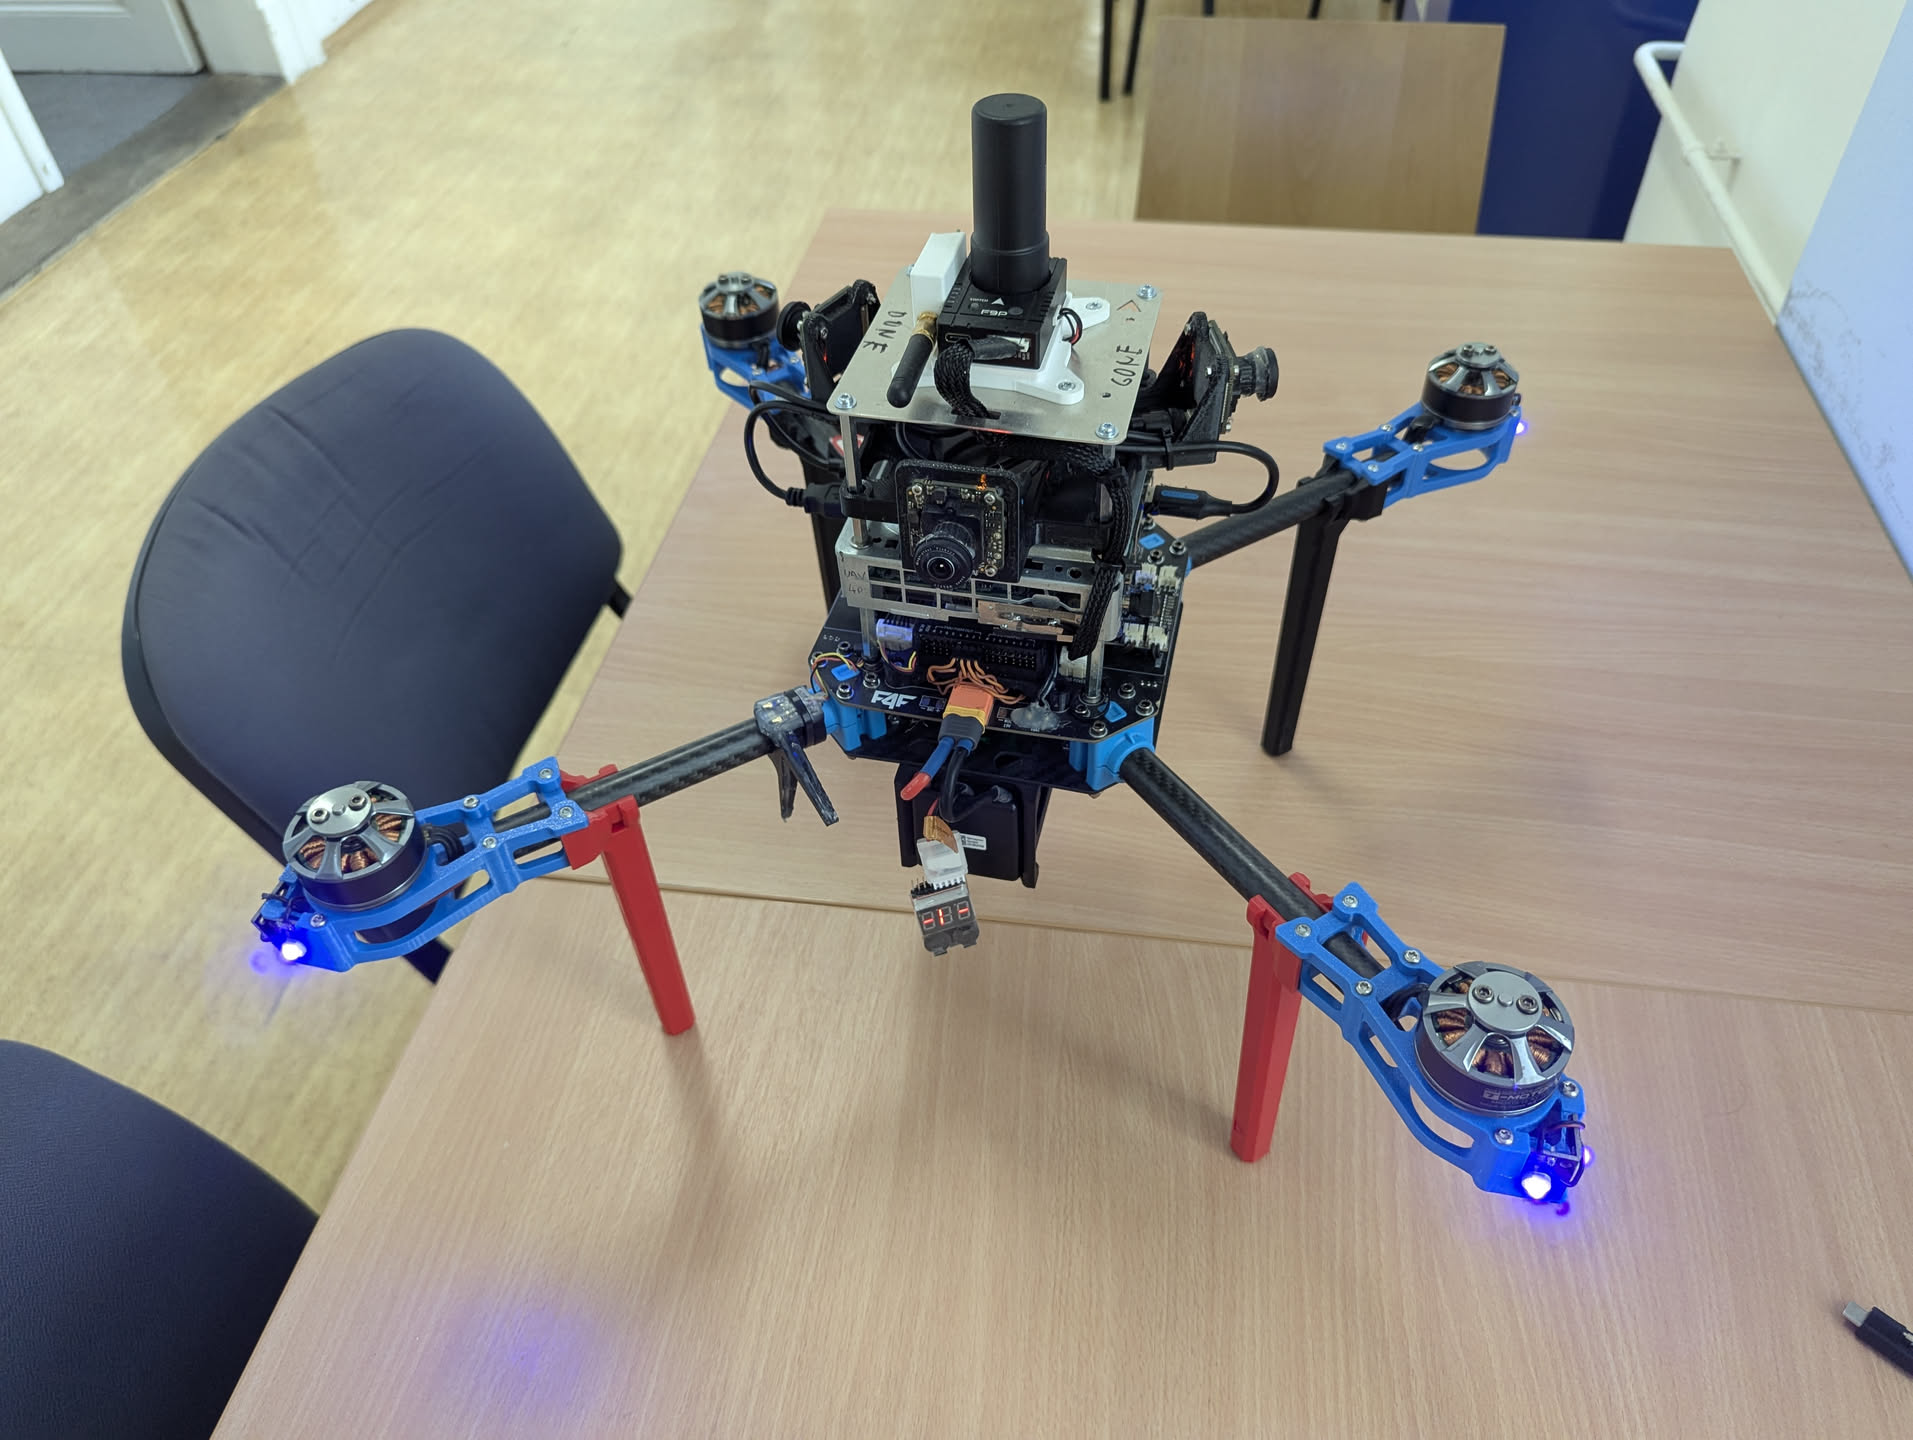
\includegraphics[width=0.50\textwidth]{./fig/photos/uav1.jpeg}
%    \caption{
%        The MRSX500 UAV
%    }
%    \label{fig:x500uav}
%\end{figure}

\subsection{Event-based camera}
The event-based camera used in this thesis is the \texttt{Prophesee EVK4 HD}\footnote{Prophesee EVK4 HD website: \url{https://www.prophesee.ai/event-camera-evk4/}.}\cite{propheseeevk4},
with \texttt{IMX636} sensor. The camera features a resolution of $1280 \times 720$ pixels and is capable of generating $1.066\times10^9$ events per second (equivalent to $10.000$ \ac{FPS} in conventional frame-based terms) and offers a dynamic range of $120$ dB.
During recording, many camera settings can be changed, such as the \ac{ROI} settings and the bias settings.
%\begin{figure}[H]
%    \centering
%    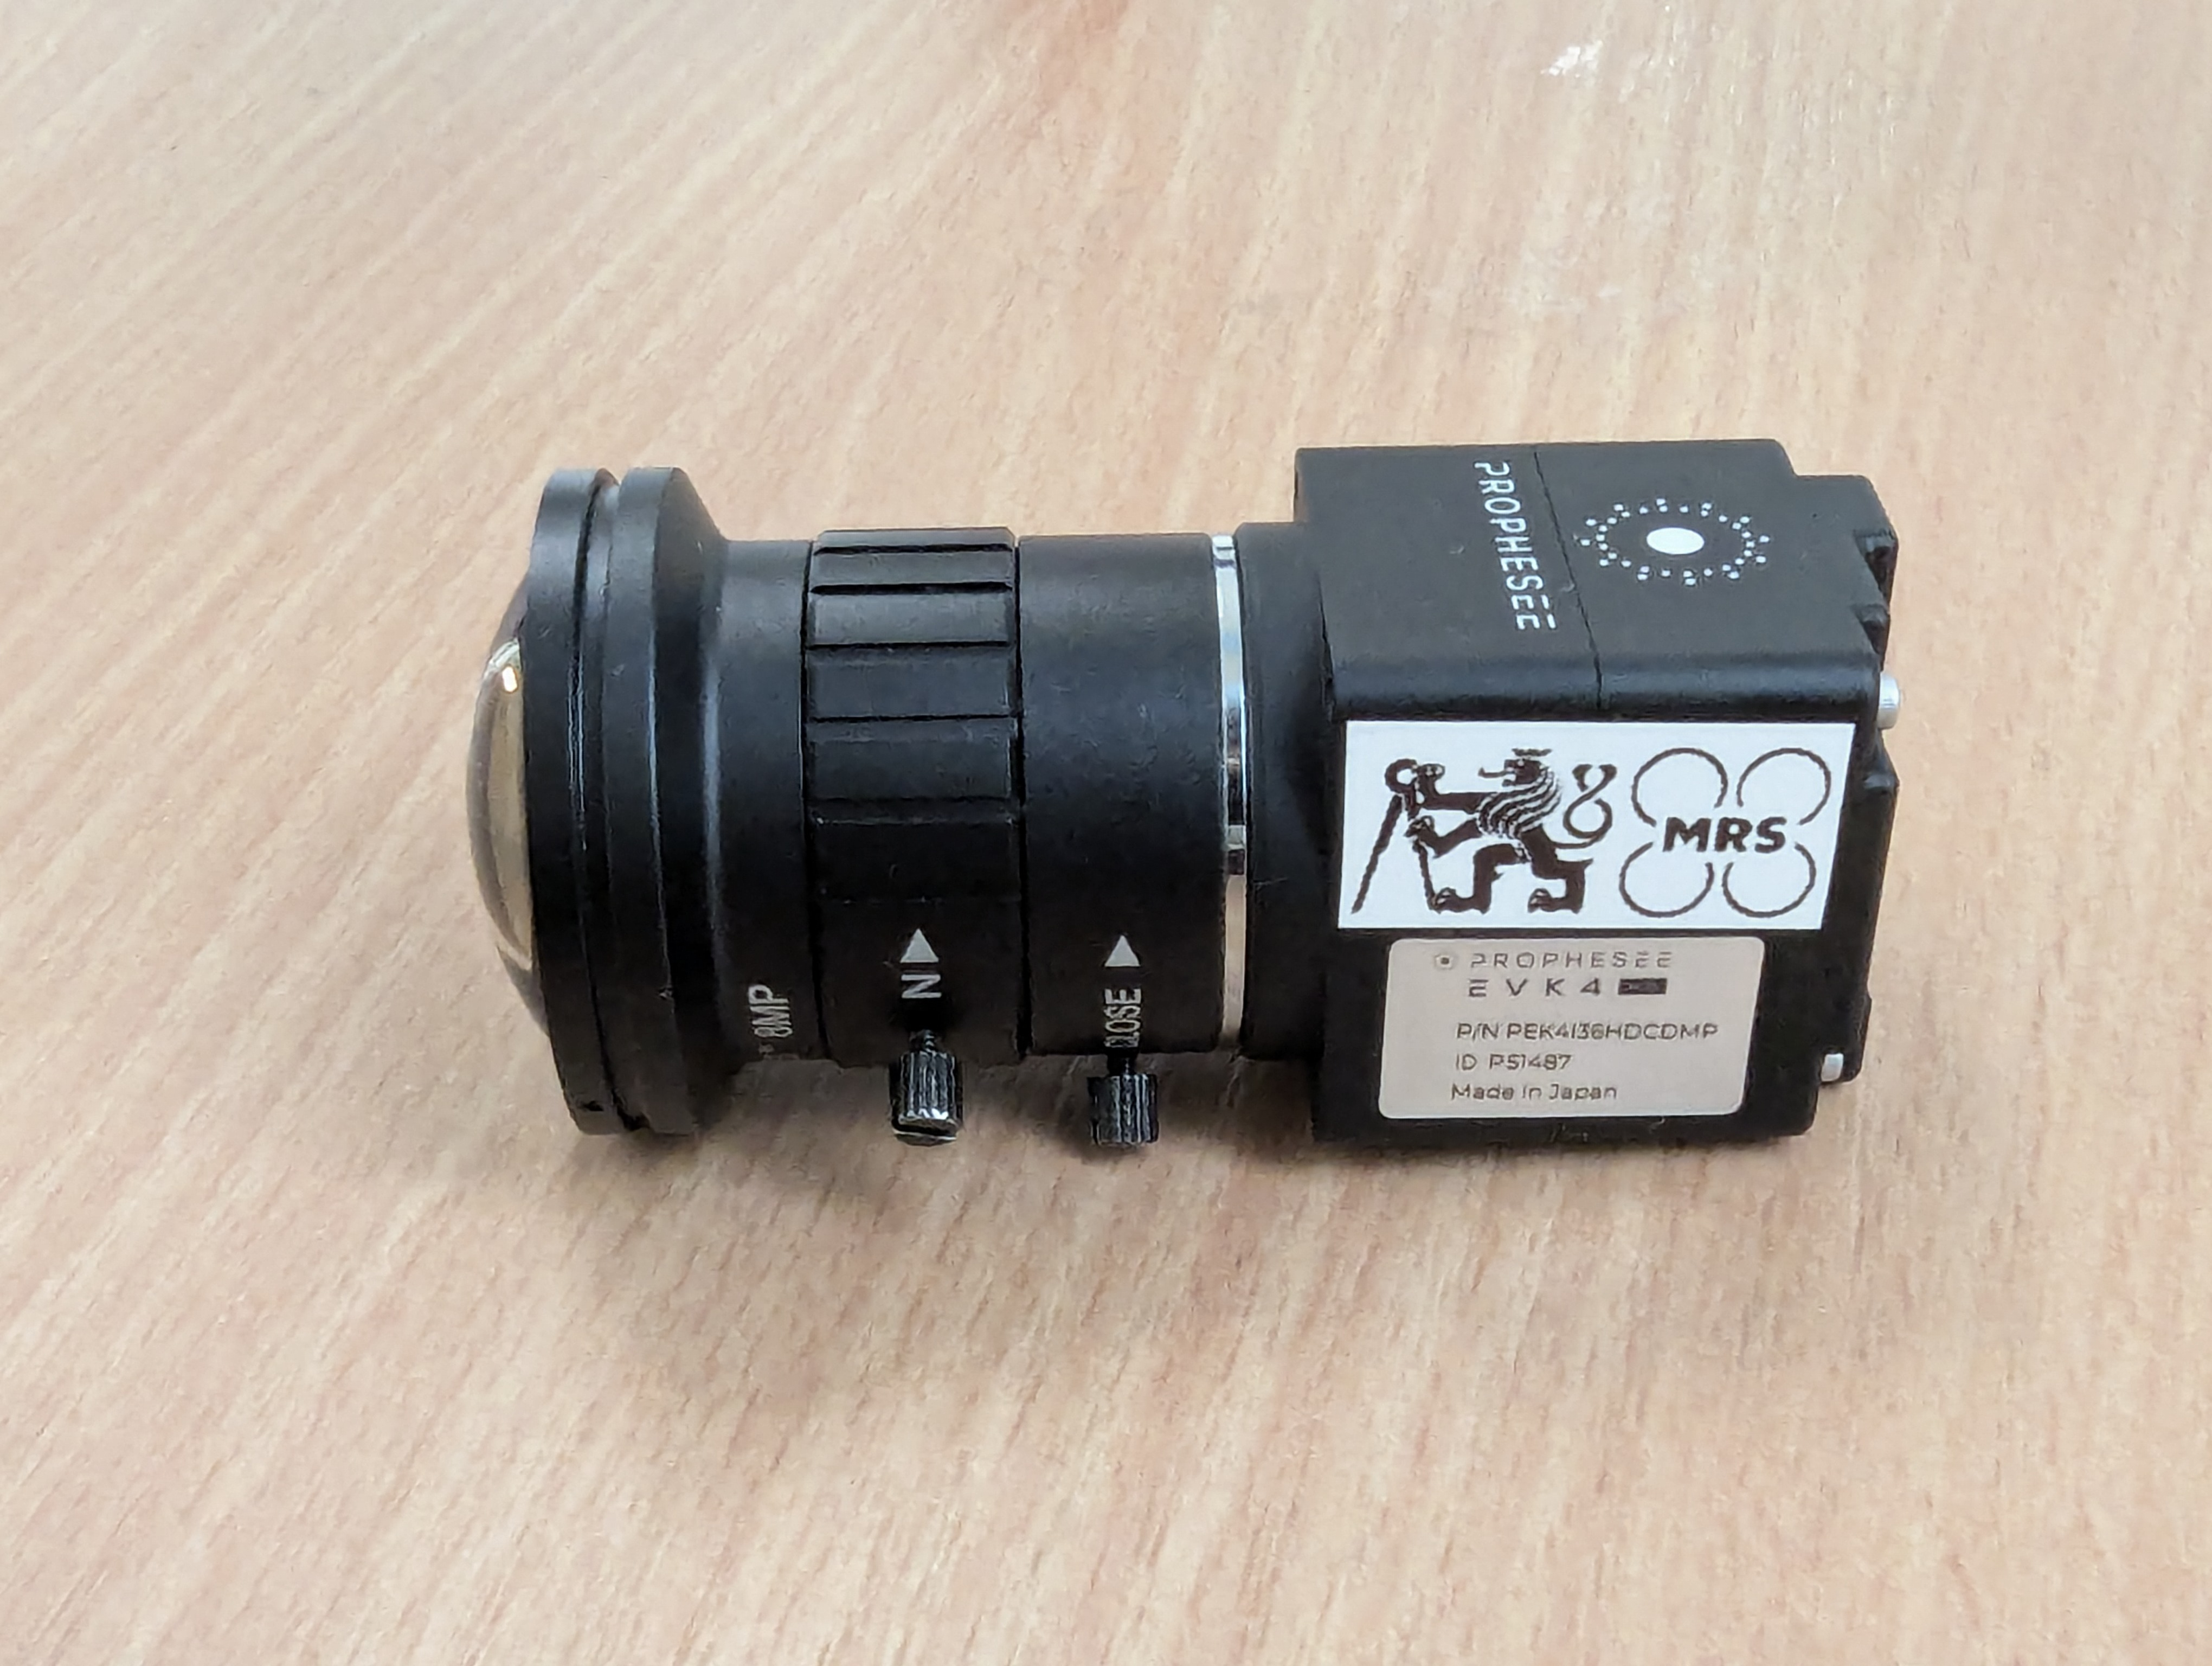
\includegraphics[width=0.50\textwidth]{./fig/photos/evk4.jpg}
%    \caption{
%        Prophesee EVK4 HD event-based camera
%    }
%    \label{fig:evk4}
%\end{figure}

\begin{figure}[H]
	\centering
	\subfloat[The event-based camera EVK4 from Prophesee with a 2.5mm fish eye lens.] {
	  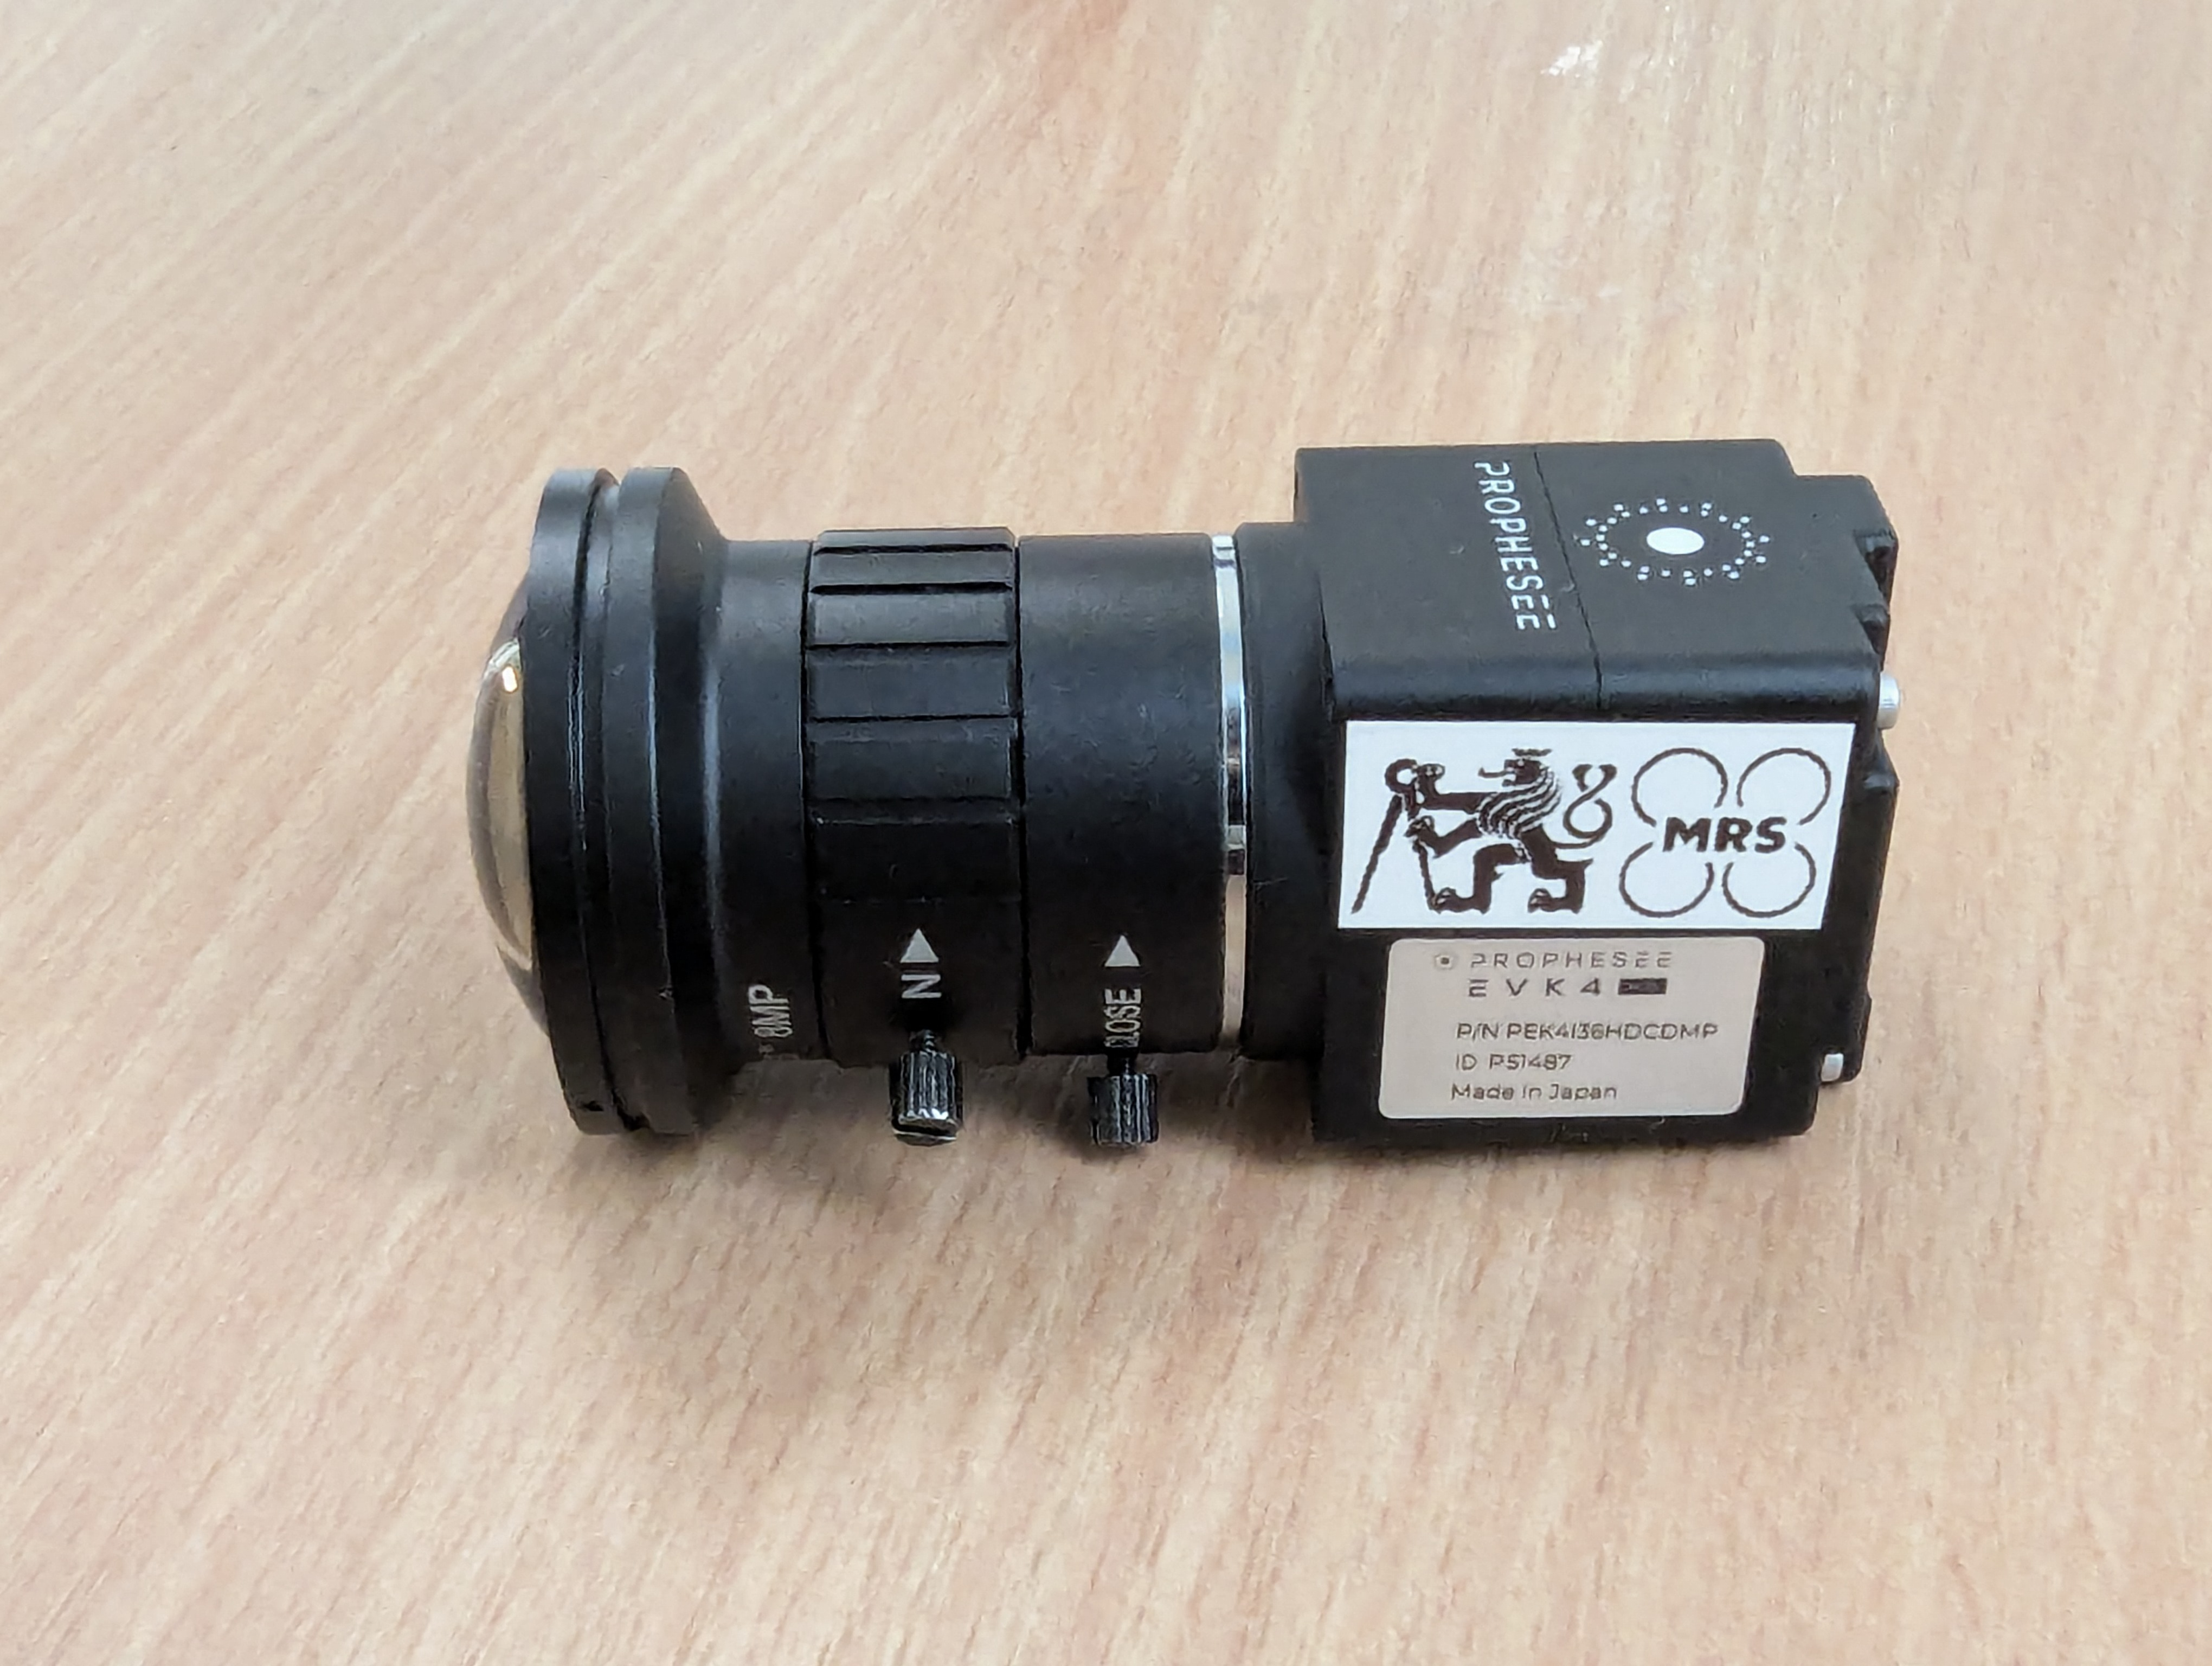
\includegraphics[width=0.5\textwidth]{./fig/photos/evk4.jpg}
	  \label{fig:evk4}
	}
	\subfloat[X500 UAV unit equipped with UVDAR] {
	  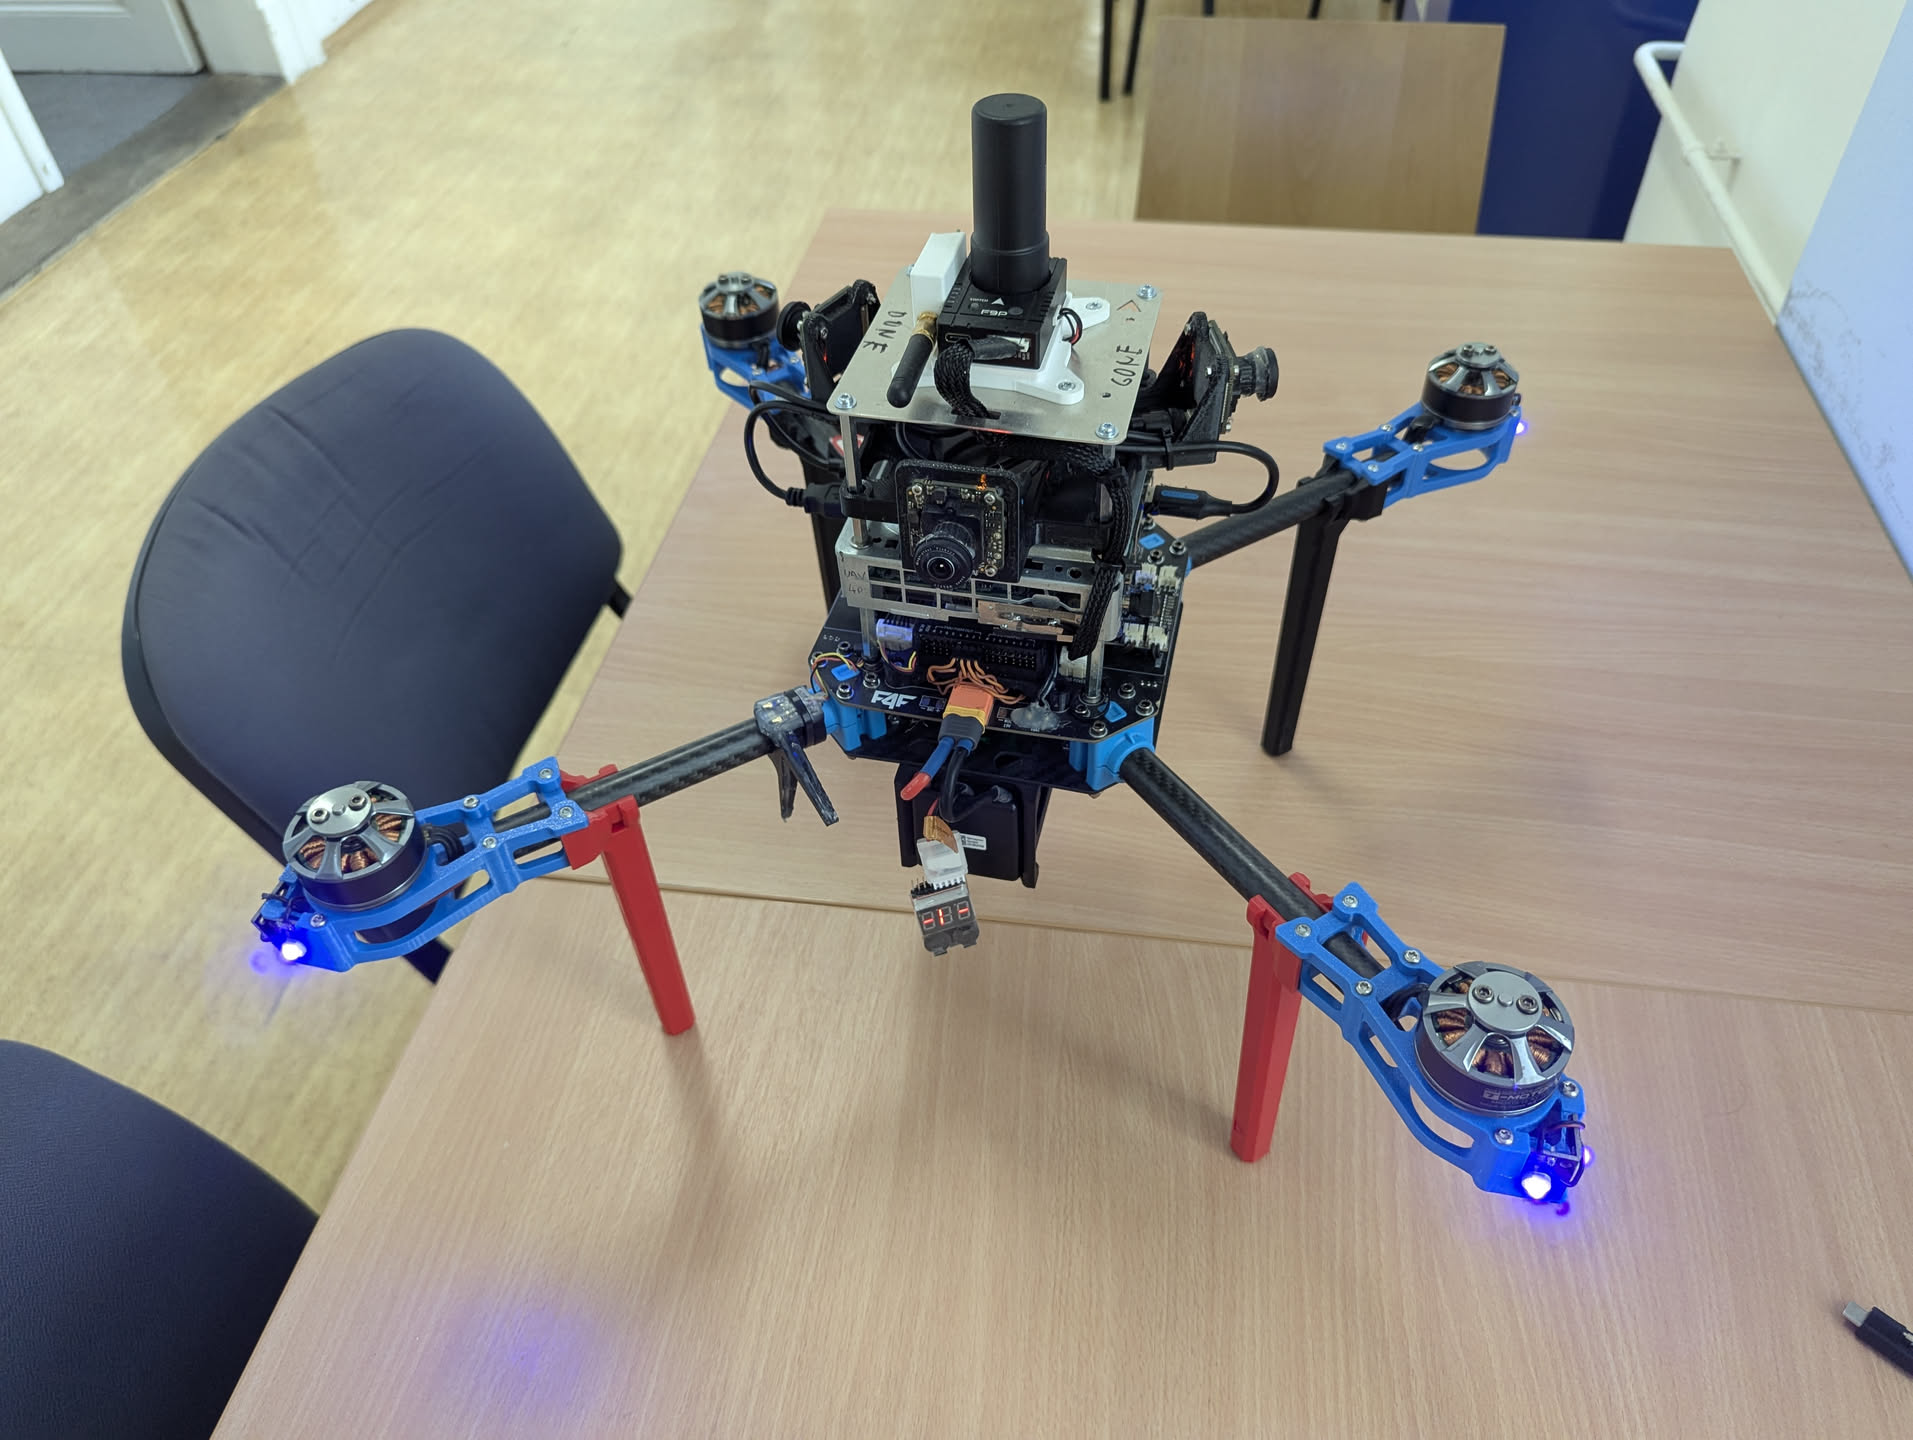
\includegraphics[width=0.5\textwidth]{./fig/photos/uav1.jpeg}
	  \label{fig:uav1}
	}
	\caption{
  An event-based camera with a 2.5mm fish eye lens can be seen on \reffig{fig:evk4}, which was used to measure the UV LEDs mounted on the X500 UAV unit modulated using UVDAR as seen on \reffig{fig:uav1}.
  }
	\label{fig:uavcam}
\end{figure}

\subsubsection{ROI}
The \ac{ROI} setting during recording takes a rectangular region in pixel coordinates and discards events outside the specified region at the hardware level, reducing computational load and noise from irrelevant areas. This setting is especially useful in cases where only a small static area needs to be observed or where many unrelated events
may be generated, that would interfere with the measurement process.

\subsubsection{Bias settings}
The bias settings are a global camera setting parameters analogous to ISO or exposure time in traditional cameras, though they operate on fundamentally
different principles.
The configurable biases for the \texttt{EVK4} which directly influence event generation and noise filtering, are as follows\cite{dilmaghani2022controlevaluationeventcameras}
\begin{itemize}
    \item \texttt{bias\_diff\_on} adjusts the threshold on which events are generated, with higher setting, the more increasing change in pixel brightness needs to be present to trigger a generation of an event with positive $\sigma$
    \item \texttt{bias\_diff\_off} adjusts the threshold on which events are generated, with higher setting, the more decreasing change in pixel brightness needs to be present to trigger a generation of an event with negative $\sigma$
    \item \texttt{bias\_fo} adjusts the low-pass filter, which filters out the fast fluctuations in light intensity, effectively setting the maximum detectable oscillation frequency
    \item \texttt{bias\_hpf} adjusts the high-pass filter, which filters out the slow fluctuations in light intensity, setting the minimum detectable oscillation frequency
    \item \texttt{bias\_refr} adjusts the pixel refractory period, in which a pixel is inactive after generating an event
\end{itemize}
These settings were optimized during data acquisition to suppress noise and extraneous events (such as from wall reflections or scene illumination changes), which
ensures that only events related to the experiment are captured.

\subsection{Lenses}
During the measurements, a $2.5$mm f/$1.6$ fish eye lens with a \ac{FOV} of $187$ degrees was used. Subsequently, during the final experiment, an ultra-wide $1.07$mm f/$2.8$ fish eye lens from Entaniya with \ac{FOV} of $280$ degrees was used in combination with the first lens.
Both lenses were equipped with narrowband \ac{UV} filters which target the specific wavelength of the \ac{LED}s that are used in the UVDAR localization system.
This ensures, that the majority of generated events come from the \ac{LED} sources mounted at the \ac{UAV}s, and less events come from the surrounding area.
All lenses were properly calibrated (see \refchap{chap:calib}), which is required to provide correct results in the final pose estimation.

\section{Data collection}

\subsection{Baseline}

The baseline experiment involved a static event camera mounted on a tripod, observing a stationary \ac{UAV} positioned at distances ranging from
$0.5$ m to $2.5$ m under controlled indoor lighting. The \ac{UAV}'s \ac{LED} markers were programmed to emit pulses of \ac{UV} light with modulation
frequencies ranging from $1$ Hz to $30$ kHz. No \ac{ROI} constraints were applied during these recordings.
This preliminary experiment revealed critical problems in the measuring technique:
\begin{itemize}
    \item Multiple visible \ac{LED}s: The camera captures the scene as a whole, with no isolation of individual light sources. This means that the results
    would not have a correct representation of a single light source, but would be influenced by other light sources from the remaining \ac{UAV}
    arms as well.
    \item Reflection artifacts: Reflections from walls and objects present in the scene are working as event-generating light sources, bouncing the light around,
    as seen on \reffig{fig:meas1}.
    This may confuse some blob detection algorithms for automatic \ac{LED} source location detection, which would be used in the analysis.
    \item Capturing of the whole scene: As the whole scene was captured, more post-processing would need to be done to analyze the recorded data and investigate
    the relations of measured effects, for example a local \ac{ROI} filter could be applied to \ac{LED} centers detected by
    a blob detection algorithm.
\end{itemize}

%This first experiment proved to be rather inefficient as the \ac{LED}s need to be isolated from each other's influence, which
%was not done properly at this time. This problem is partially solvable in the post-processing, by filtering out the events
%with \ac{ROI} filter usage (it is possible to filter the events by finding bounding boxes
%that encapsulate light sources, but on a more complex scene this approach becomes relatively hard).
%The other issue turned out to be the reflections of surrounding objects (as seen in \reffig{fig:meas1}), which caused
%another source of unwanted events in the recording, which may in turn confuse some blob detection methods.

\begin{figure}[H]
	\centering
	\subfloat[An event-camera view of the UAV with UV LEDs.] {
	  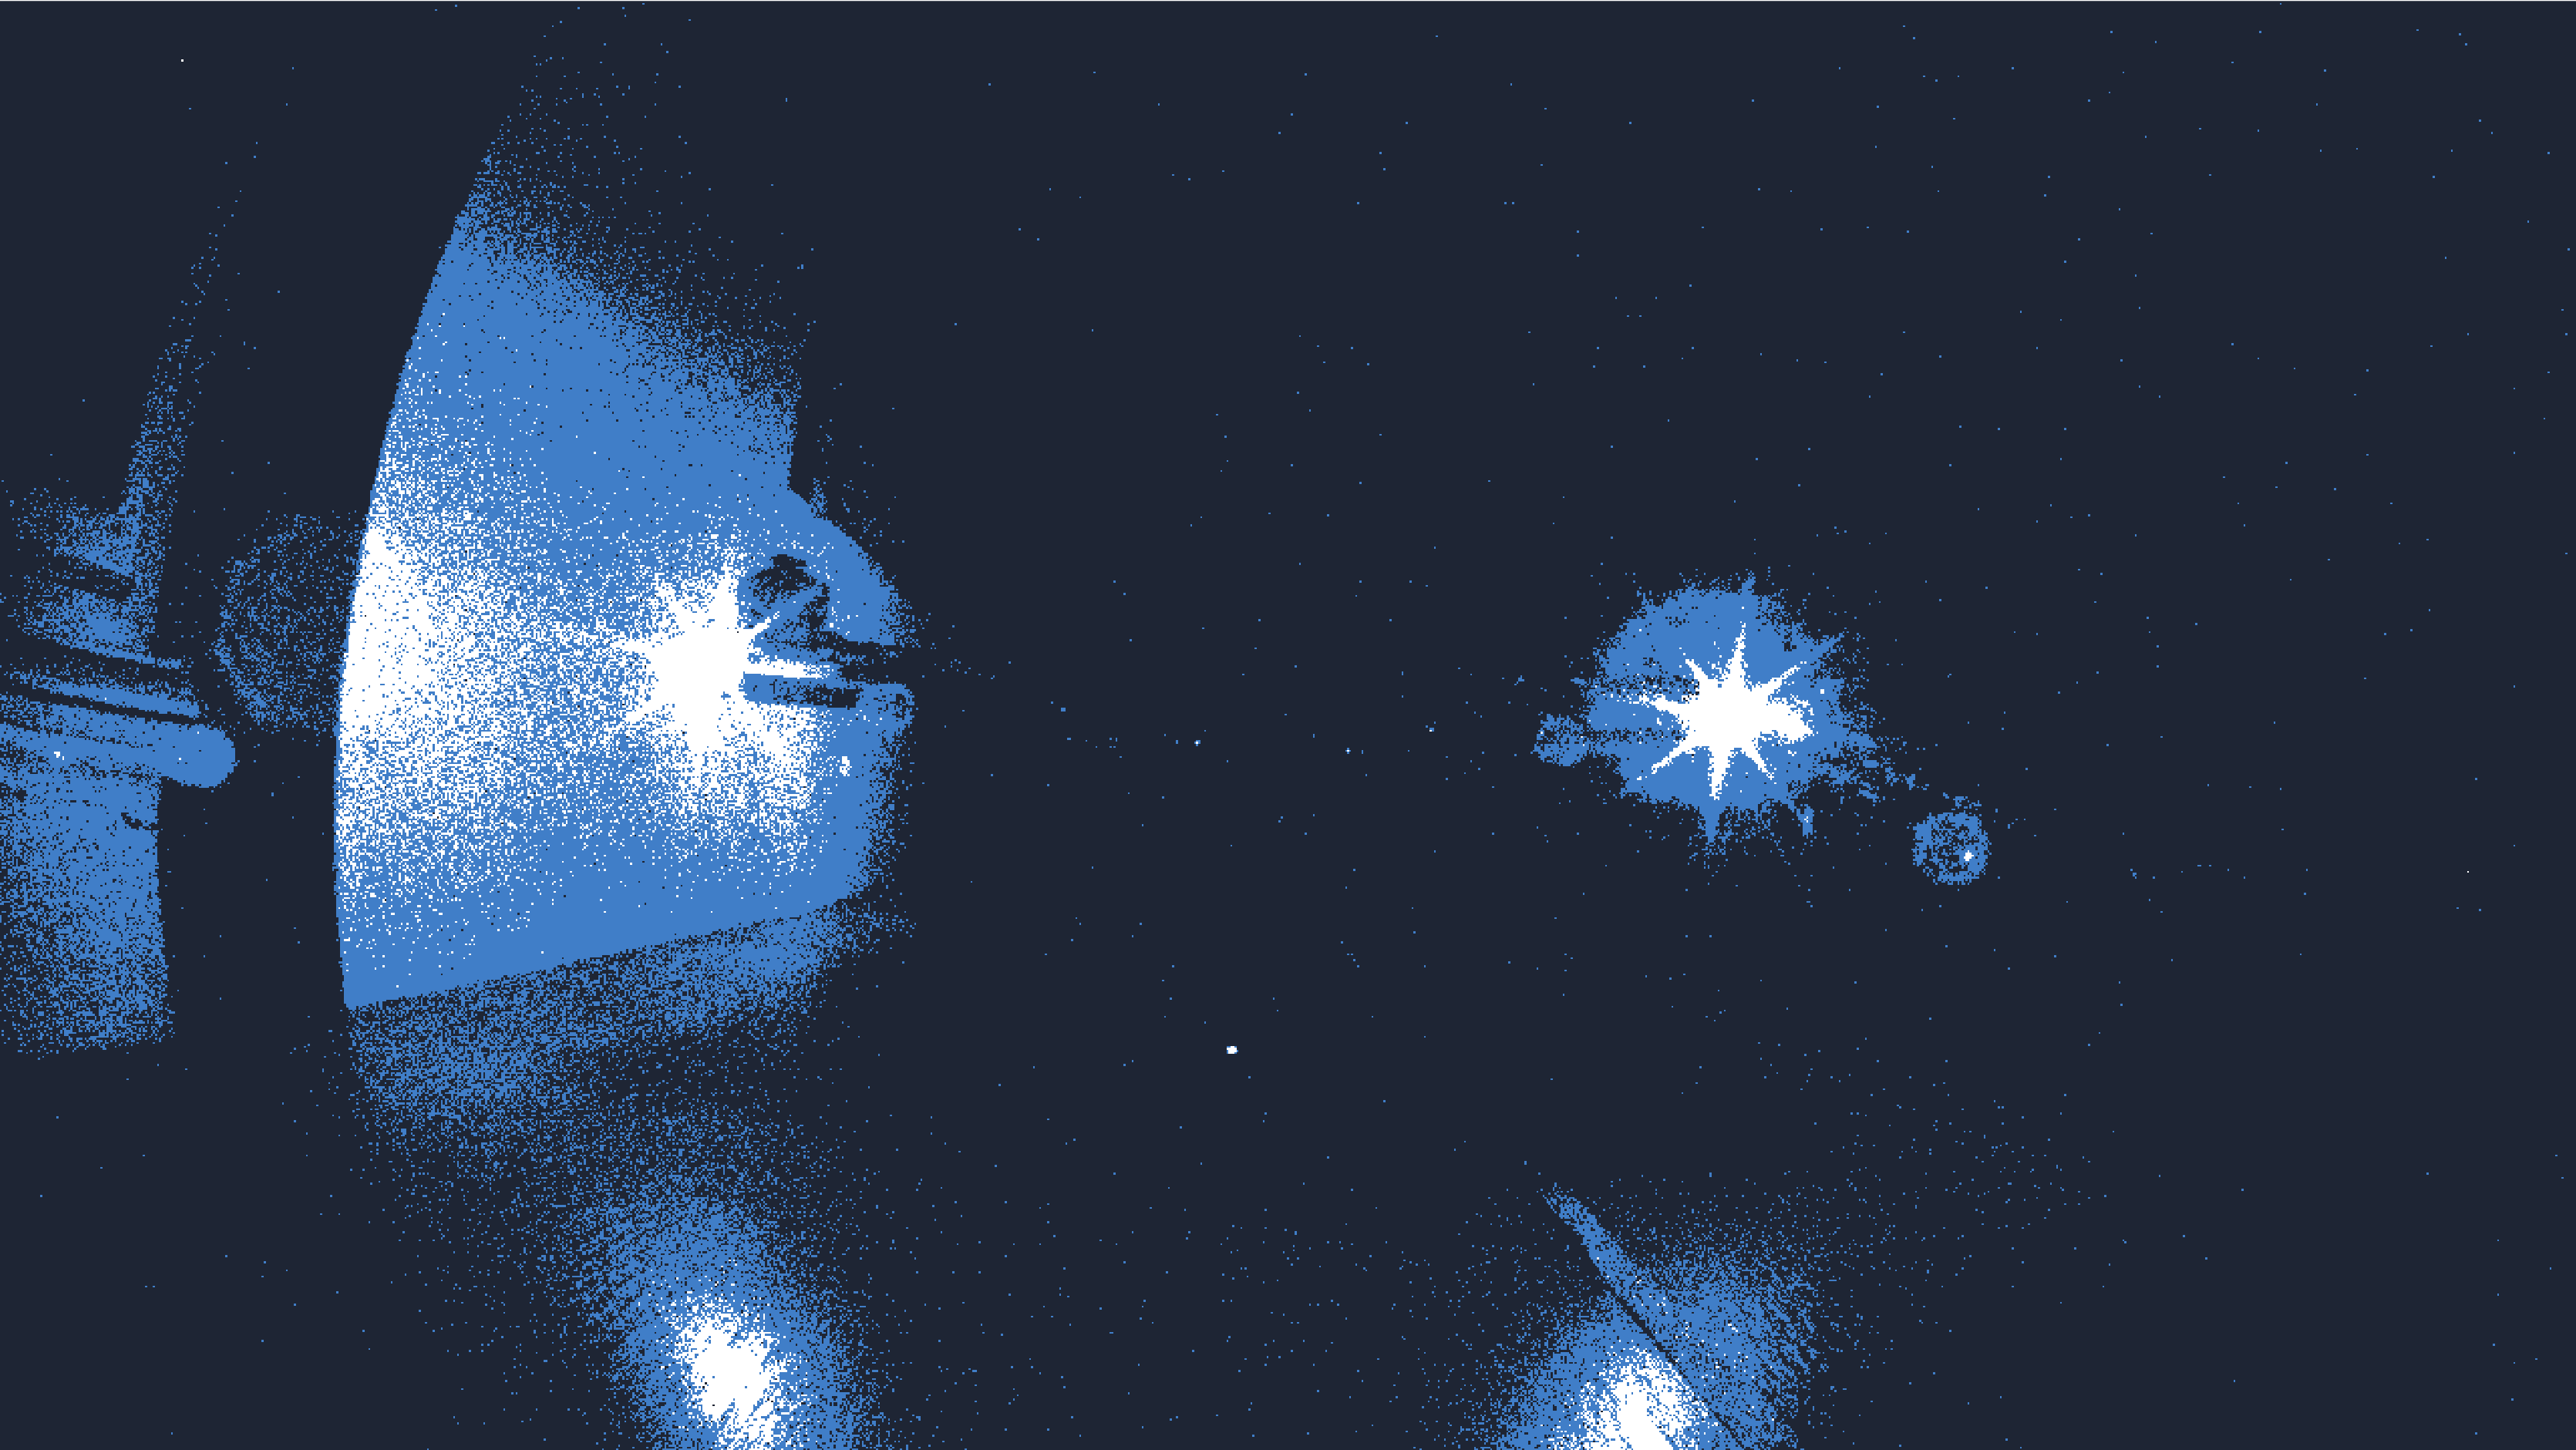
\includegraphics[width=0.5\textwidth]{./fig/photos/meas1.png}
	  \label{fig:meas1_e}
	}
	\subfloat[View of the experiment setup.] {
	  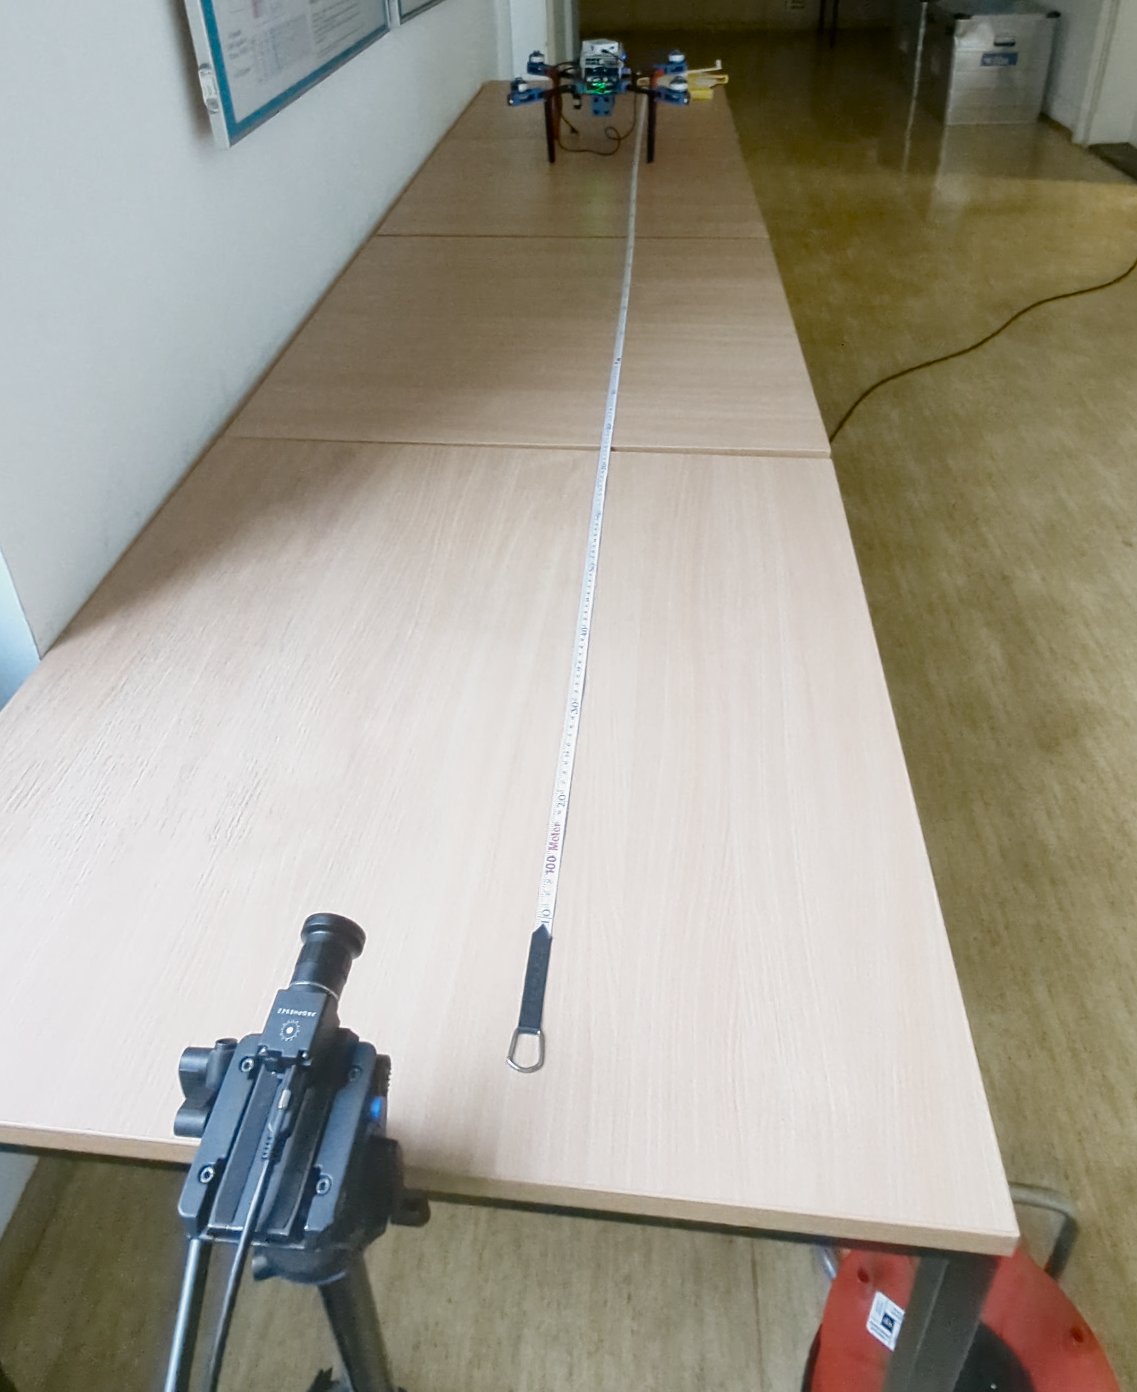
\includegraphics[width=0.5\textwidth]{./fig/photos/meas1_c.png}
	  \label{fig:meas1_c}
	}
	\caption{
  The setup for measuring the event-camera response with a EVK4 camera. Visible reflections from a wall can be seen on \reffig{fig:meas1}. The setup is shown on \reffig{fig:meas1_c}.
  }
	\label{fig:meas1}
\end{figure}


\subsection{Distance - frequency influence}

With the critical problems revealed in the previous experiment, only one light source consisting of 2 \ac{UV} \ac{LED}s at the end of the \ac{UAV} arm was turned on and
modulated at set frequencies.
Measurements were made in areas isolated by \ac{ROI} filter directly during recording on the hardware level, events were collected only in the
selected area around the and of the \ac{UAV} arm.
This time, the position of the \ac{UAV} was fixed relative to the camera on a blank background, with no wall reflections. The camera was placed on a tripod
and moved in increments of $0.2$ meters, starting from $1$ meter and ending at $3$ meters, with additional measurements made
at $4$ and $5$ meters.
The frequency range of the LED modulation was set in a range of $10$ Hz to $30$ kHz, with the blinking sequence set to \texttt{0, 1}.

\subsection{Rotation angle influence}

In addition to distance and frequency influence, the rotation angle influence also needs to be considered, to
verify the emitting characteristics of the light sources - if they can or cannot be considered Lambertian.
The \ac{UAV} was rotated at increments of $45$ degrees relative to the event-based camera, at distances of $0.5$, $1$ and $2$ meters,
with frequencies ranging from $10$ Hz to $10$ kHz and the blinking sequence was set to \texttt{0, 1}.

%\subsection{RSSR Data collection}

%TODO: Rewrite this section

%Another dataset was collected for the application of \ac{RSSR} \cite{sooyongrssr}, which we analyze more in \refchap{chap:rssr}.
%The data includes calibration data, which is necessary for the optical system parameter estimation. This calibration is done by
%recording a video using a calibration lattice of LEDs with known spacing, and observing the pattern distortion in the
%resulting video.
%The UAV was placed at increasing distances and various angles relative to the event-based camera, with the LEDs blinking at frequencies different from
%each other. 
%The blinking sequences were set to the following values:
%\begin{lstlisting}
%	led_1 = [0, 0, 0, 0, 0, 0, 0, 0, 1, 1, 1, 1, 1, 1, 1, 1]
%	led_2 = [0, 0, 0, 0, 1, 1, 1, 1, 0, 0, 0, 0, 1, 1, 1, 1]
%	led_3 = [0, 0, 1, 1, 0, 0, 1, 1, 0, 0, 1, 1, 0, 0, 1, 1]
%	led_4 = [0, 1, 0, 1, 0, 1, 0, 1, 0, 1, 0, 1, 0, 1, 0, 1]
%\end{lstlisting}
%with a common modulation frequency of $250$ Hz.
%This allows for the measurement of the ratio
%explain why to use the ratio, not the absolute value
%\footnote{Using the absolute value of the LED power is not suitable, as it also depends of the camera settings, surrounding
%environment and other factors. Finding such ratio (or property) that stays constant is crucial for correct distance estimation.}
%between the responses for each of the LEDs, which is necessary
%for the estimation of the UAV position using RSSR.

\section{Response analysis}

The event-based camera response data was analyzed using the Metavision SDK\footnote{Metavision SDK Docs: \url{https://docs.prophesee.ai/stable/index.html}}
using its Python API. Each recording can be loaded as a raw file, producing a structured Numpy array of events, where each event is structured as an array of values
$(t, x, y, p)$. Specifically, $t$ represents the time stamp from the start of the recording, $x$ and $y$ the spatial location of the event
on the camera sensor, and $p$ the polarity of the change in the detected brightness (compared to the previously recorded one).
%We can use many methods to analyze this data, such as

\subsection{Distance - frequency influence}

The distance frequency data set has recordings of the \ac{UAV} placed in front of the camera at distances $\mathcal{D}$ with one \ac{LED} being modulated
at frequencies $\mathcal{F}$ \footnote{The frequencies represented in this list are the actual frequencies sent to the UVDAR unit. The preserved frequencies
are half of the values in this list - UVDAR interprets the frequency with a reference to the length of the sequence (here the sequence being \texttt{[0, 1]}).}.
%To minimize interference, only one LED was active during each recording, enabling isolated characterization of the diode’s response.
The tested ranges were:
\[
\mathcal{F} = \{10, 25, 50, 100, 250, 500, 1000, 2500, 5000, 10000, 20000, 30000\} \, \text{Hz},
\]
\[
\mathcal{D} = \{1.0 + 0.2k \mid k \in \{0, \dots, 10\}\} \cup \{4.0, 5.0\} \, \text{m}.
\]
%\begin{lstlisting}
%frequencies_Hz = [10, 25, 50, 100, 250, 500, 1000, 2500, 5000, 10000, 20000, 30000]
%distances_m = [1.0, 1.2, 1.4, 1.6, 1.8, 2.0, 2.2, 2.4, 2.6, 2.8, 3.0, 4.0, 5.0]
%\end{lstlisting}
We can load the obtained data set into a matrix representing the distances and frequencies, then load a select number of events from each recording.
The data is then resampled into a signal, represented by a 1D array obtained from summing polarities $p_i$ over a selected bin width $\Delta t$
\footnote{The bin width should be adjusted appropriately, as the farther the event-based camera is from the source, the fewer events are generated.} \refeq{eq:signal}.
\begin{equation}
    S[k] = \sum_{i\in\mathcal{B}_k}p_i, \quad \mathcal{B}_k=\{i|t_k\leq t_i<t_k+\Delta t\}
    \label{eq:signal}
\end{equation}
Peaks in this signal are then analyzed by SciPy's \texttt{findpeaks} function,
and the average number of events with the standard deviation is calculated for each frequency and distance.
We can see the influence of distance and frequency on the average number of events in \reffig{fig:dist} and \reffig{fig:freqs}, respectively. The data show a decreasing trend of the average number of events
with the increase of distance or frequency. The drop related to the distance can be explained by the perceived decrease in the intensity of the light source with increasing distance. With an increasing frequency, the camera cannot capture
all the changes that are generated by the light source, leading to a perceived drop in brightness.
On very high frequencies and distances, the camera is not able
to detect any real events at all, as there is more noise generated by the camera itself at this point. This can be observed
at \reffig{fig:dist} with a frequency of $30$ kHz at $3$ meters.

%\begin{figure}[H]
%	\centering
%	\subfloat[Influence of distance on the average number of events.] {
%	  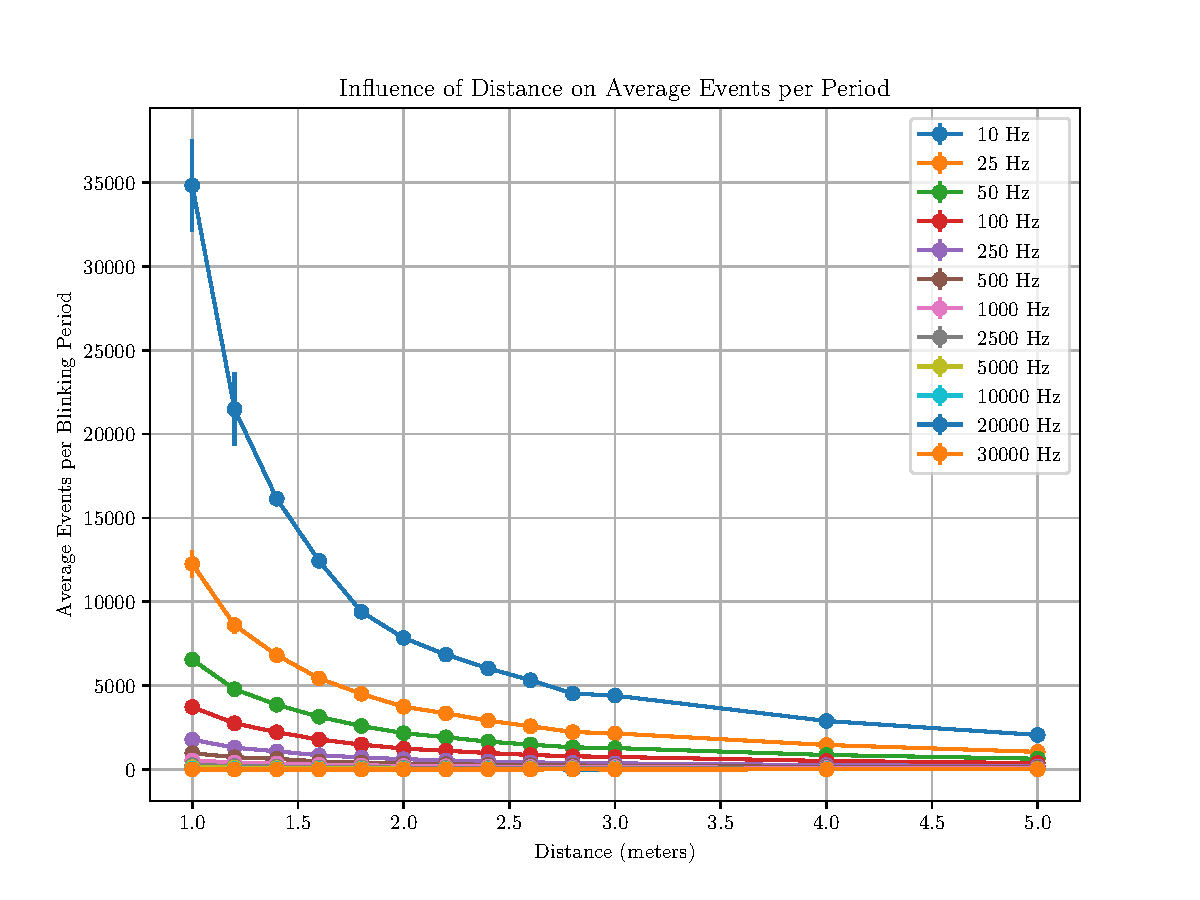
\includegraphics[width=0.5\textwidth]{./fig/semestral/dist.pdf}
%	  \label{fig:dist_1}
%	}
%	\subfloat[Influence of distance on the log of average number of events.] {
%	  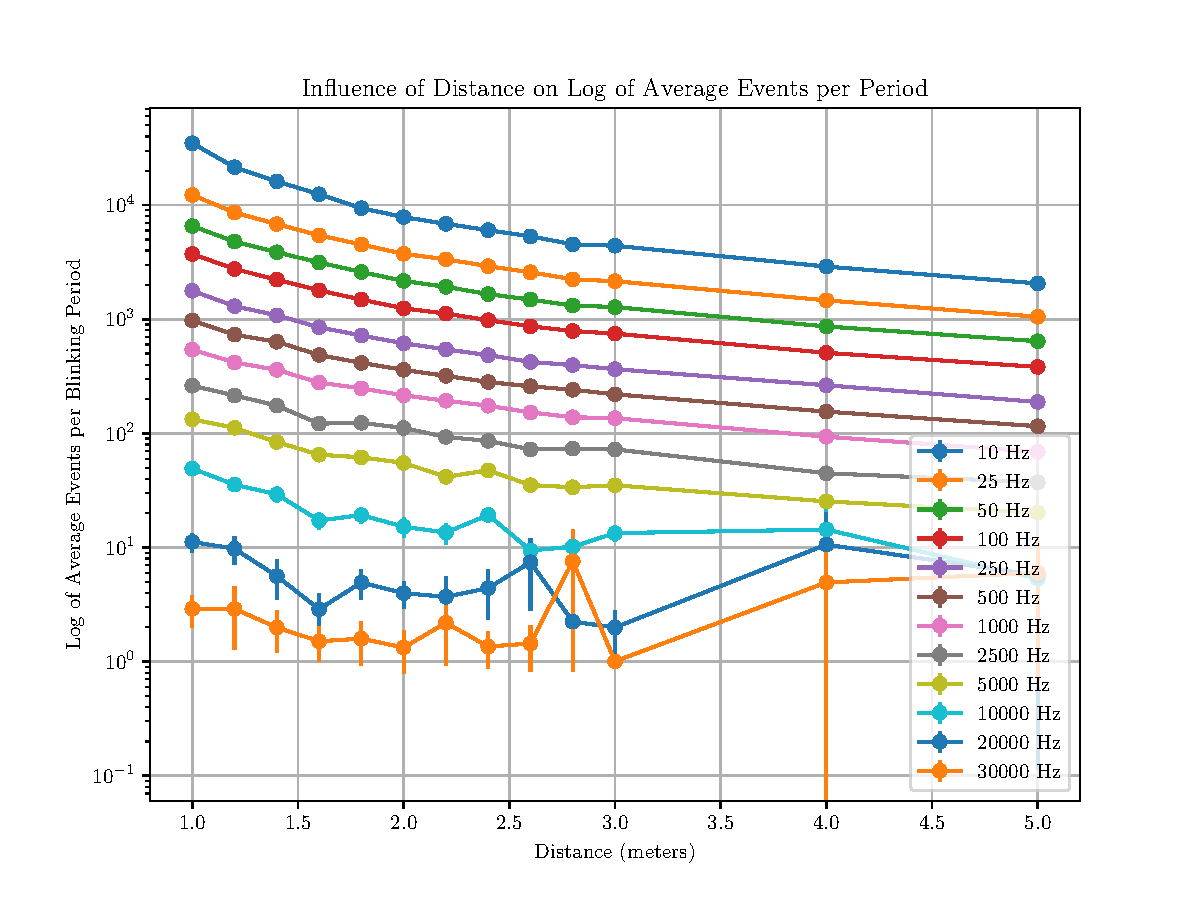
\includegraphics[width=0.5\textwidth]{./fig/semestral/distlog.pdf}
%	  \label{fig:dist_2}
%	}
%	\caption{
%  The influence of distance on the average number of events with the UAV rotated 0 degrees relative to the event-based camera on \reffig{fig:dist_1}, and with the log of the average number of events on \reffig{fig:dist_2}.
% }
%	\label{fig:dist}
%\end{figure}
%\begin{figure}[H]
%	\centering
%	\subfloat[Influence of frequency on the average number of events.] {
%	  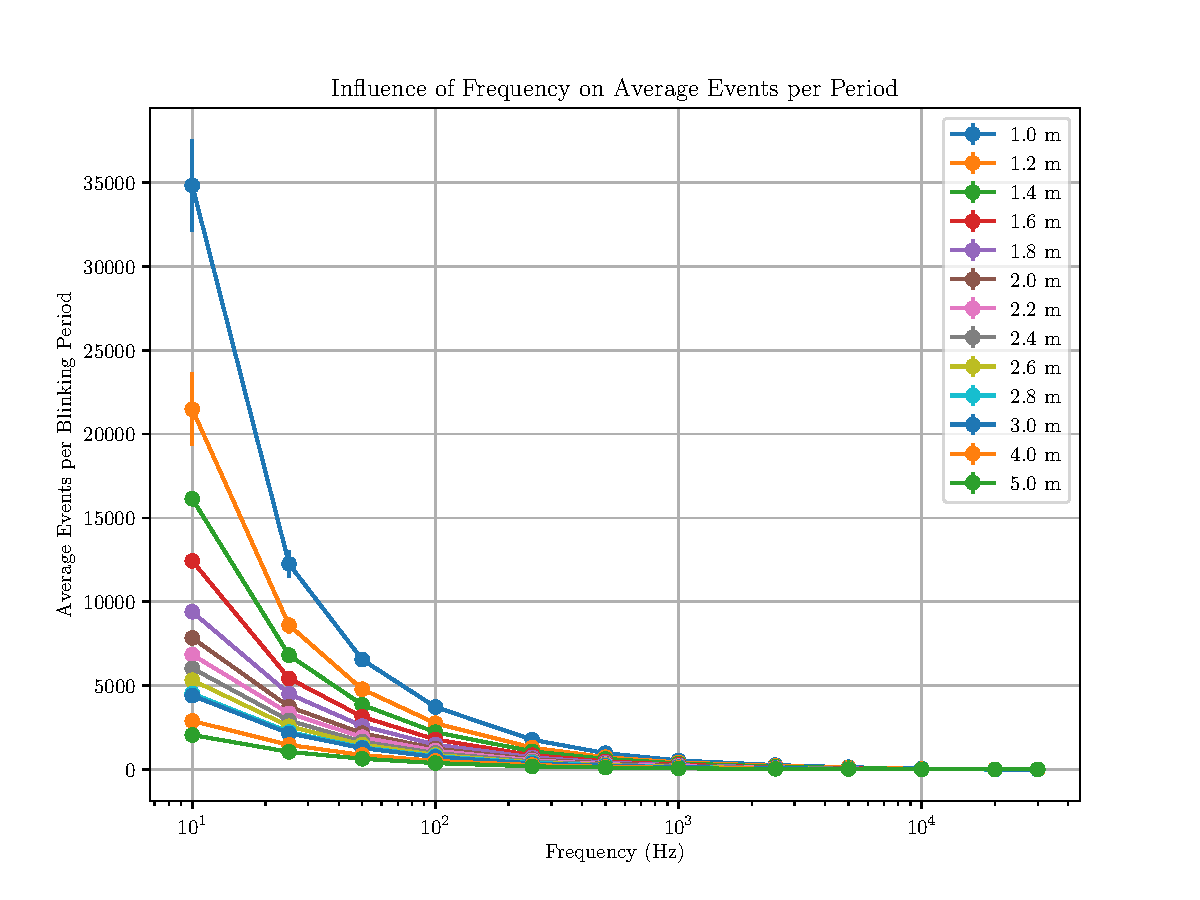
\includegraphics[width=0.5\textwidth]{./fig/semestral/freq.pdf}
%	  \label{fig:freqs_1}
%	}
%	\subfloat[Influence of frequency on the log of average number of events.] {
%	  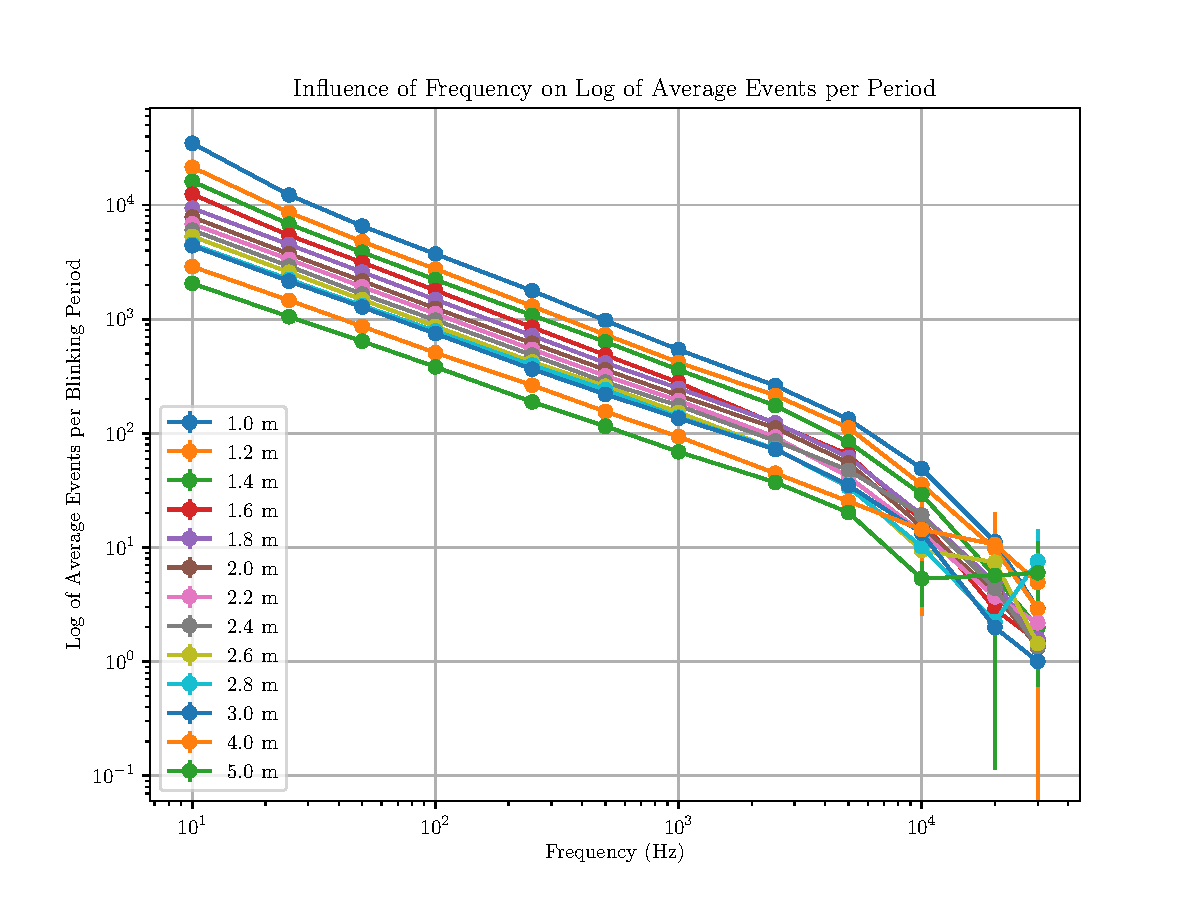
\includegraphics[width=0.5\textwidth]{./fig/semestral/freqlog.pdf}
%	  \label{fig:freqs_2}
%	}
%	\caption{
%  The influence of frequency on the average number of events with the UAV rotated 0 degrees relative to the event-based camera on \reffig{fig:freqs_1}, and with the log of the average number of events on \reffig{fig:freqs_2}.
%  }
%	\label{fig:freqs}
%\end{figure}

\begin{figure}[H]
    \centering
    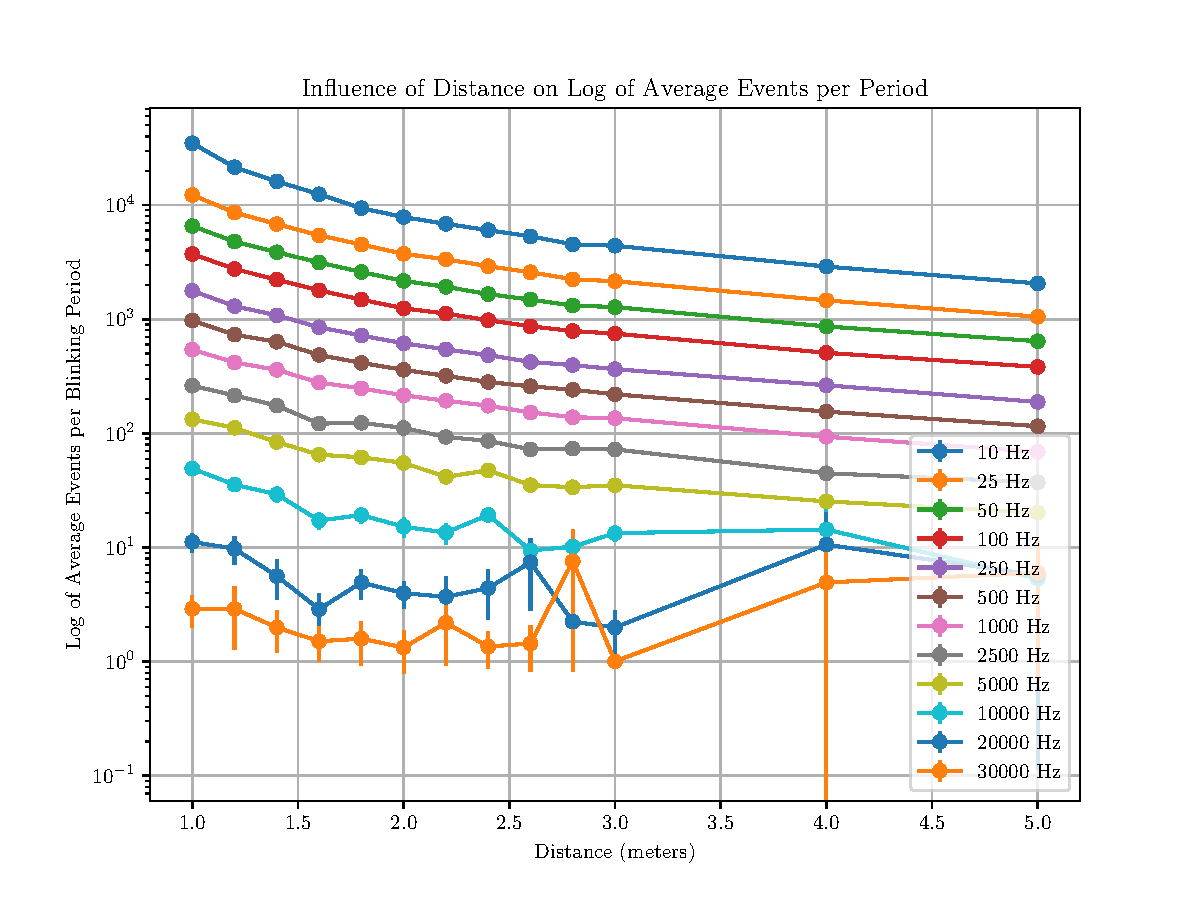
\includegraphics[width=0.85\textwidth]{./fig/semestral/distlog.pdf}
    \caption{
        Influence of distance on the log of the average number of events, with the UAV rotated 0 degrees relative to the event-based camera.
    }
    \label{fig:dist}
\end{figure}

\begin{figure}[H]
    \centering
    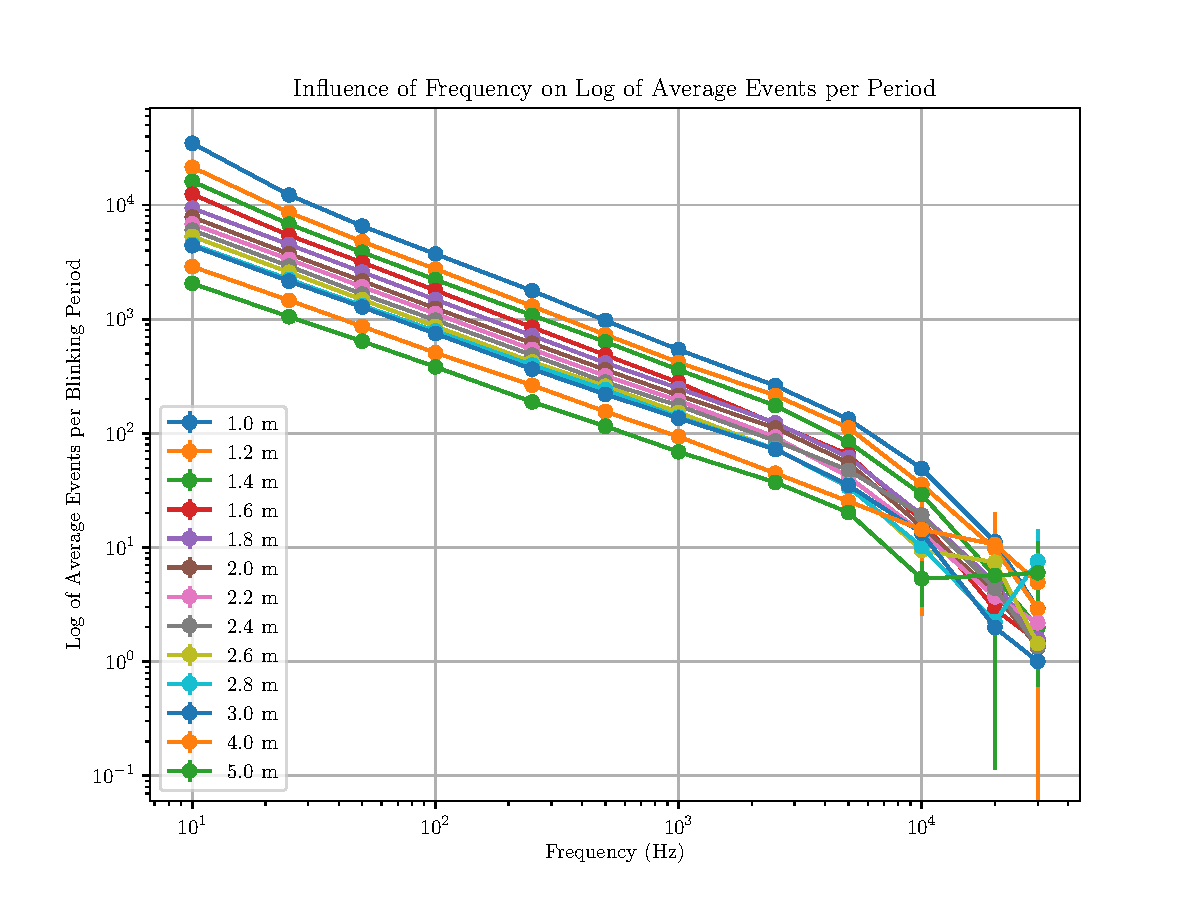
\includegraphics[width=0.85\textwidth]{./fig/semestral/freqlog.pdf}
    \caption{
        Influence of frequency on the log of the average number of events, with the UAV rotated 0 degrees relative to the event-based camera.
    }
    \label{fig:freqs}
\end{figure}
If we now select one frequency and try to fit it with a curve,
we can observe that the data can be approximated with a rational or an exponential function, as shown in \reffig{fig:fit1}.
The best fit without being too complex is the inverse square law, which can be expressed as
\begin{equation}
	\text{intensity} \propto \frac{1}{\text{distance}^2}
\end{equation}
While more complex functions could be used to fit the data, they would likely lead to overfitting rather than capturing the underlying trend in a generalizable way, thus the inverse square law provides a good approximation of the data.
\begin{figure}[H]
	\centering
	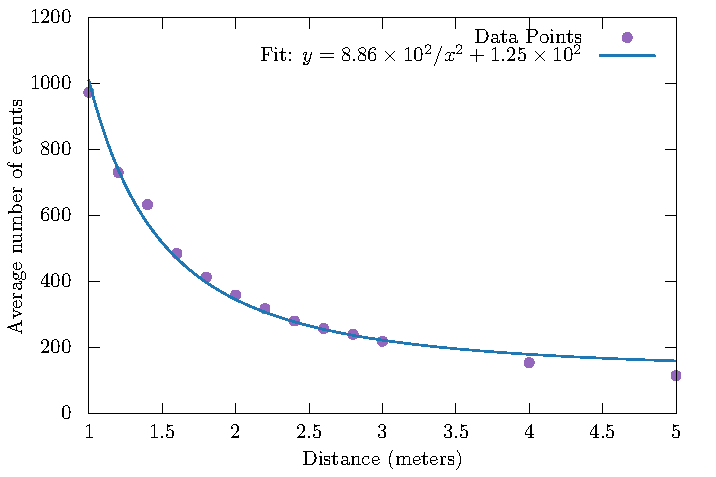
\includegraphics[width=0.80\textwidth]{./fig/semestral/inverse_square/square.pdf}
	\caption{Influence of distance data fitted with various curves.}
	\label{fig:fit1}
\end{figure}

\subsection{Rotation angle influence}
From the manufacturers datasheet of the used ProLight PM2B-1LLE 1W \ac{UV} Power \ac{LED} \footnote{The datasheet of ProLight PM2B-1LLE 1W UV Power LED can be obtained from \url{https://www.tme.eu/Document/9dfb498784ffdd07892a42f4f17c6f37/PM2B-1LLE-DTE.pdf}}
used in the UVDAR system, we can learn that the \ac{LED}s have a Lambertian radiation pattern,
which can be seen on \reffig{fig:lambertian}.
\begin {figure}[H]
	\centering
	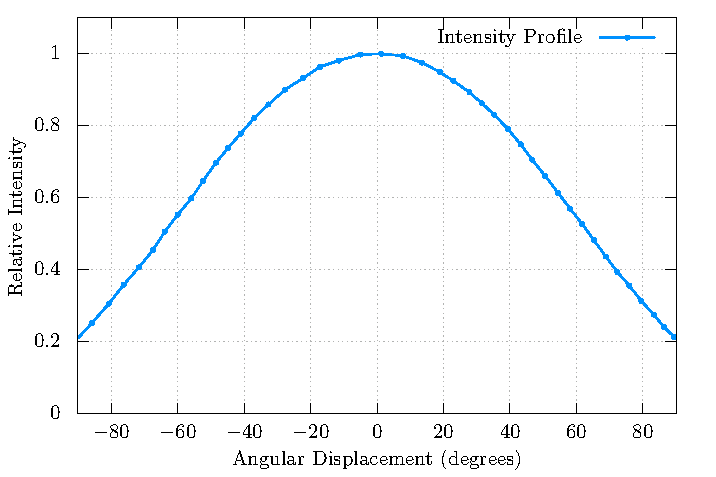
\includegraphics[width=0.75\textwidth]{./fig/semestral/lambertian/_new_lambertian.pdf}
	\caption{Lambertian radiation pattern of the PM2B-1LLE UV LED.}
	\label{fig:lambertian}
\end{figure}
This means that the intensity of the light emitted from the LED decreases with the cosine
of the angle between the normal of the LED and the direction of the light \refeq{eq:lambertian}.
\begin{equation}
	I(\theta) = I_0\cos(\theta)
	\label{eq:lambertian}
\end{equation}
To represent the whole end of the \ac{UAV} arm, we need to consider two \ac{LED} sources, orthogonal to each other.
This can be represented by shifting the previous distributions by $\pm 45$ degrees and adding them together. The 
theoretical distribution pattern of the light source is visible in \reffig{fig:lambert_combined}. 
The results extracted from the dataset of the \ac{UAV} rotations relative to the camera are shown in \reffig{fig:angles}.
%With the dataset of the rotation of the UAV relative to the camera we will get the following resultson \reffig{fig:angles}.
\begin {figure}[H]
	\centering
	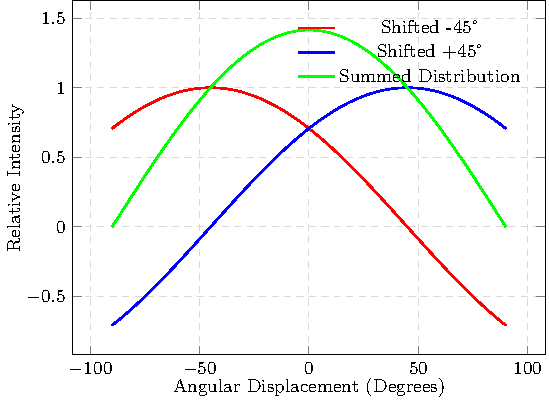
\includegraphics[width=0.50\textwidth]{./fig/semestral/lambertian/3lambertian.pdf}
	\caption{Radiation pattern of two lambertian light sources shifted by $\pm 45$ degrees.}
	\label{fig:lambert_combined}
\end{figure}

\begin{figure}[H]
	\centering
	\subfloat[Influence of rotation of the UAV on the log of average number of events at 0.5 m.] {
	  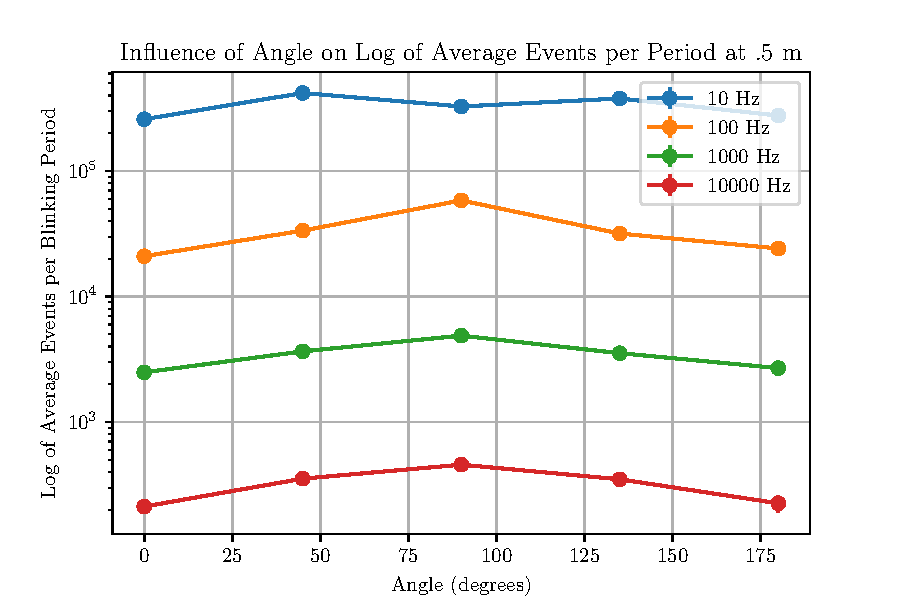
\includegraphics[width=0.5\textwidth]{./fig/semestral/angle1.pdf}
	  \label{fig:angle_1}
	}
	% \subfloat[Influence of rotation of the UAV on the log of average number of events at 1 m.] {
	%   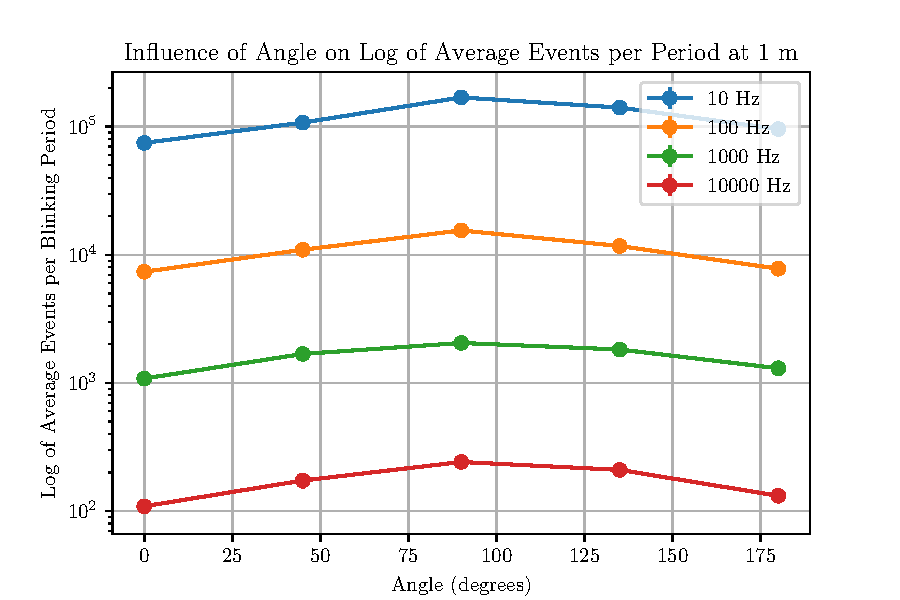
\includegraphics[width=0.5\textwidth]{./fig/semestral/angle2.pdf}
	%   \label{fig:angle_2}
	% }
	\subfloat[Influence of rotation of the UAV on the log of average number of events at 2 m.] {
	  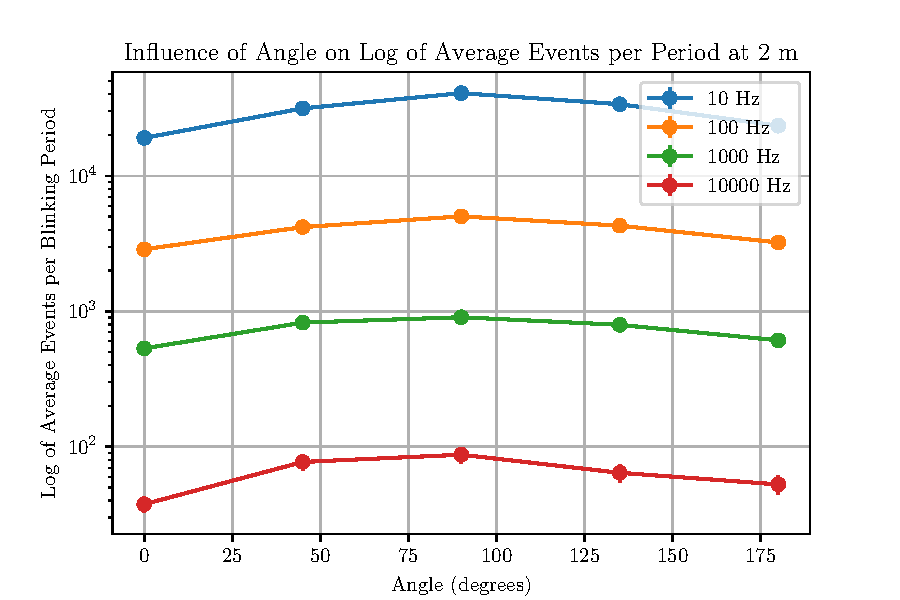
\includegraphics[width=0.5\textwidth]{./fig/semestral/angle3.pdf}
	  \label{fig:angle_3}
	}
	\caption{
  The influence of rotation angle on the log of average number of events at 0.5 m on \reffig{fig:angle_1} and at 2 m on \reffig{fig:angle_3}.
  }
	\label{fig:angles}
\end{figure}
The data show a rough approximation of the theoretical distribution on \reffig{fig:lambert_combined},
but with a drop of intensity at the middle of the distribution. This could be caused
by the fact that LEDs, when close to the camera, can be perceived as multiple light sources,
but when moved further away, they merge into one source as shown on \reffig{fig:leds}.

\begin{figure}[H]
	\centering
	\subfloat[2 LEDs with blinking frequency of 10 Hz at 0.5 m.] {
	  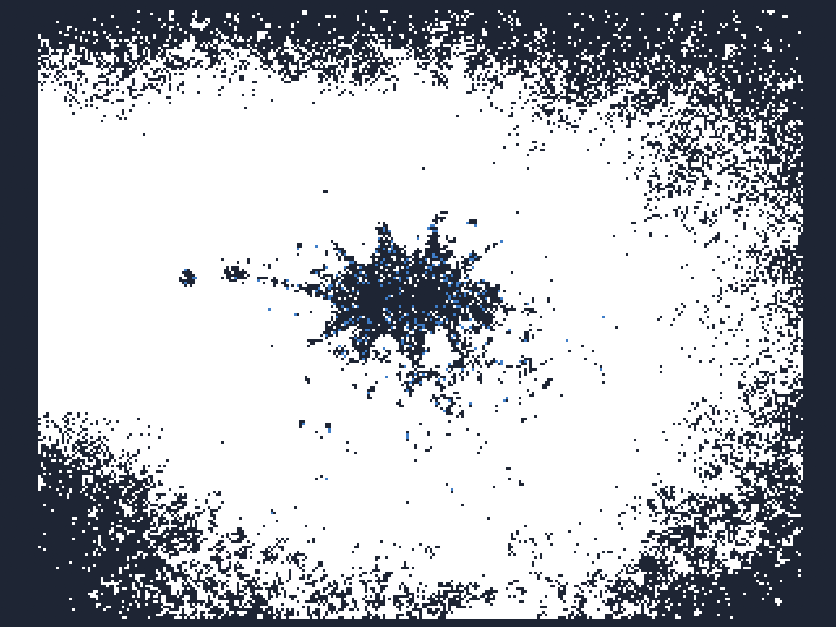
\includegraphics[width=0.5\textwidth]{./fig/photos/2leds_05m.png}
	  \label{fig:leds_1}
	}
	\subfloat[2 LEDs with blinking frequency of 10 Hz at 2 m.] {
	  
\includegraphics[width=0.5\textwidth]{./fig/photos/2leds_2m.png}
	  \label{fig:leds_2}
	}
	\caption{
  The light source on one arm of the UAV, consisting of two UV LEDs, blinking at a frequency of 10 Hz,
  placed at 0.5 m on \reffig{fig:leds_1} and 2 m at \reffig{fig:leds_2}.
  }
	\label{fig:leds}
\end{figure}
What we can also observe from \reffig{fig:leds} are the star-like shapes of the LEDs, which are supposed to be circular.
Those shapes are caused by light diffraction (and are named diffraction spikes), which are, in turn, caused by the aperture
blades in the lens of the camera. The number
of star spikes depend on the number of blades, the set aperture and the light source intensity then causes stars of different
levels of profoundness.\cite{lendermann2018computational} We can observe this by comparing how profound the star shapes are on different
frequencies, as shown on \reffig{fig:stars}.

\begin{figure}[H]
	\centering
	\subfloat[LED blinking at 10 Hz at 1.0 m] {
	  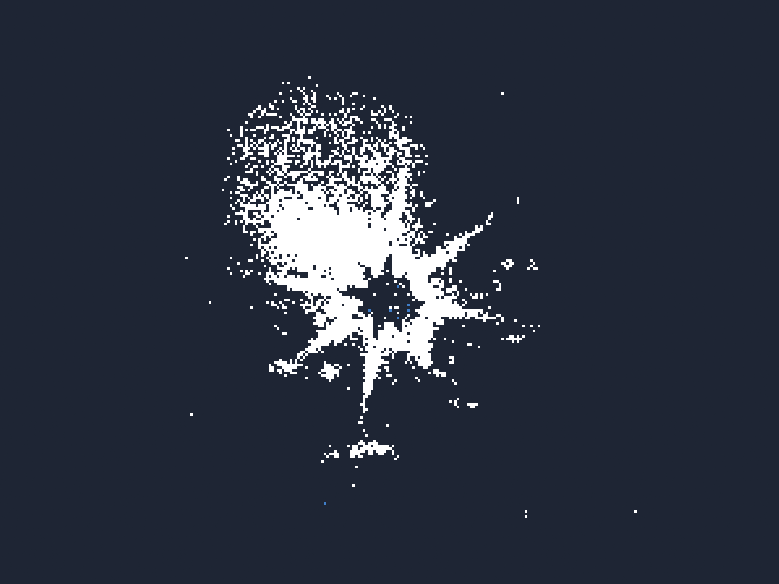
\includegraphics[width=0.5\textwidth]{./fig/photos/led_10hz.png}
	  \label{fig:stars_1}
	}
	\subfloat[LED blinking at 1 kHz at 1.0 m] {
	  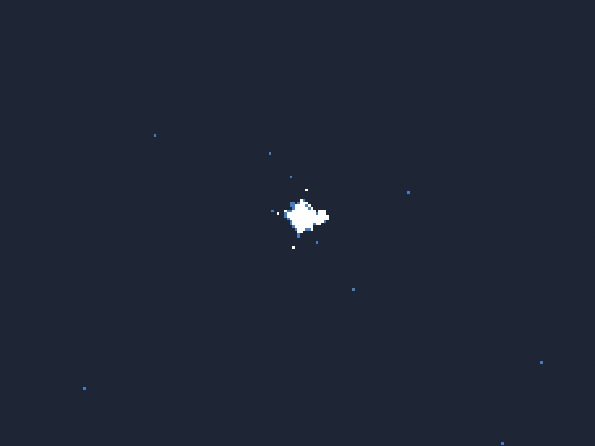
\includegraphics[width=0.5\textwidth]{./fig/photos/led_1000hz.png}
	  \label{fig:stars_2}
	}
	\caption{
  Two same LED light sources at 1.0 meters, blinking at 10 Hz and 1 kHz.
  \reffig{fig:stars_1} shows a visible diffraction star (while being much brighter), while \reffig{fig:stars_2} shows a
  much more cicular source of light that is not as bright.
  }
	\label{fig:stars}
\end{figure}